% Chapter Template

\chapter{Results and Discussion} % Main chapter title

\label{Chapter5} % Change X to a consecutive number; for referencing this chapter elsewhere, use \ref{ChapterX}

This section covers the results of the GNSS reception and GPS transmission experiments. Section \ref{sec:Res_GNSSReception} covers the attempts at receiving authentic GNSS
signals and accurately calculating a location. Section \ref{sec:Res_GPSTransmission} will cover the attempts and results of performing spoofing attacks on GPS receivers.
The overall results and trends are then discussed.
%----------------------------------------------------------------------------------------
%	SECTION 1
%----------------------------------------------------------------------------------------

\section{GNSS Reception} \label{sec:Res_GNSSReception}
Before testing the GPS transmission performance of the SDR, reception was tested, without success. Three antenna setups were chosen with each failing to lock and track the
satellites. A log linear, an omnidirectional and an active patch antenna were all used. The active antenna should have given best results since it included amplifiers
with a total gain of 28dB and
filters within the antenna module itself. The failure could be to do with the bias-t used to inject the 5V DC into the antenna, however testing with a multi-meter showed
that there was 5V on the RF+DC port of the Tee. Further testing of the bias-T and hardware setup was requried, but was not achievable due to time constraints.

%----------------------------------------------------------------------------------------
%	SECTION 2
%----------------------------------------------------------------------------------------

\section{GPS Transmission} \label{sec:Res_GPSTransmission}
% Experimentation was performed at the Tonsley campus of Flinders University, which has coordinates of $-35.007650, 138.572030$, within the Faraday cage. At first it was decided to use the
% centre of the Adelaide CBD as the coordinates for spoofing, that is $-34.5571732282, 138.3599516878$. Therefore it would be considered successful if the GPS receiver was to show
% that the current location was in the CBD. This was extended to include other locations, Davis Station in Antarctica and the MAB at Flinders University Tonsley Campus with
% coordinates of $-68.5762449235, 77.9696166515$ and $-35.00792163316667, 138.5715065625$ respectively.

Experimentation was performed from the Tonsley campus of Flinders University, which has coordinates of $-35.007650, 138.572030$, within the Faraday cage.Therefore it would
be considered successful if the GPS receiver was to show that the current location was not at this location. The chosen spoof locations were Davis Station in
Antarctica and the MAB at Flinders University Tonsley Campus with coordinates of $-68.5762449235, 77.9696166515$ and $-35.00792163316667, 138.5715065625$ respectively.
The MAB was chosen as a conveinient location to be able to test authentic and spoofed signals. The Antarctic location was chosen as an arbitrarily location that would
not be simple to get an authentic signal from, therefore a successful spoof would be easy to show.

Dynamic spoofing attacks were set to the road surrounding the MAB and around the CBD of Adelaide. The MAB was used as a small path test that would be quick to complete,
and the CBD loop was much longer taking a long time to complete the full path.


All spoof attack dates were set to the same date, which was chosen to be
the 30th March 2021. This was arbitrary and only chosen since this was when official testing began.

\subsection{Meaconing Attack}
Since the GPS reception using an SDR was unsuccessful the plan of perfoming a meaconing attack was abandonded since access to the raw received signal was recquried.
Therefore, the only viable attack strategy was to generate a binary file of the intended location. It would be ideal to perform this kind of attack in the future since
this is the only basic attack type that can be used on the encrypted military band.

\subsection{Spoofing Attack}
Once the workflow and hardware setup for the SDR was properly configured it was found that a smartphone was able to be spoofed.
When attempting to spoof devices in the wild, the Pixel XL smartphone was susceptible to attack while more modern smartphones that were tested were not susceptible. These
included the iPhone 12 Pro, Samsung Galaxy S10 and Google Pixel 3XL. The spoofing setup was not able to fool any of these devices. This could be down to software based
anti-spoofing algorithms that have been implemented including the usage of multiple constellations for position resolution.

\subsection{Static Spoofing}
\subsubsection{Tonsley MAB}
The grassed area outside of the Flinders University Tonsley campus was chosen as one of the points to spoof to. As mentioned above the desired coordinates that the receiver were
$-35.00792163316667, 138.5715065625$.

The $\frac{C}{N_0}$ ratio graph for the static MAB spoof attack, see Figure \ref{fig:MABStaticCNo}, shows that there was a good quality signal being received throughout
the test, with no evidence of under running. 
In this example the time to first fix was calculated as being 37 seconds. This is quite good for a cold start situation. During experimentation the time to first fix has
been variable between 30 seconds and 180 seconds. A trend has been the quicker the fix the better the overall accuracy of the spoofed location.
At approximately the time of first fix it can be seen that there was a reduction in number of satellite PRNs being received. Then throughout there was spikes from various
satellites. These spikes offer no benefit since they only lasted a few seconds. 

\begin{figure}[H]
    \begin{centering}
        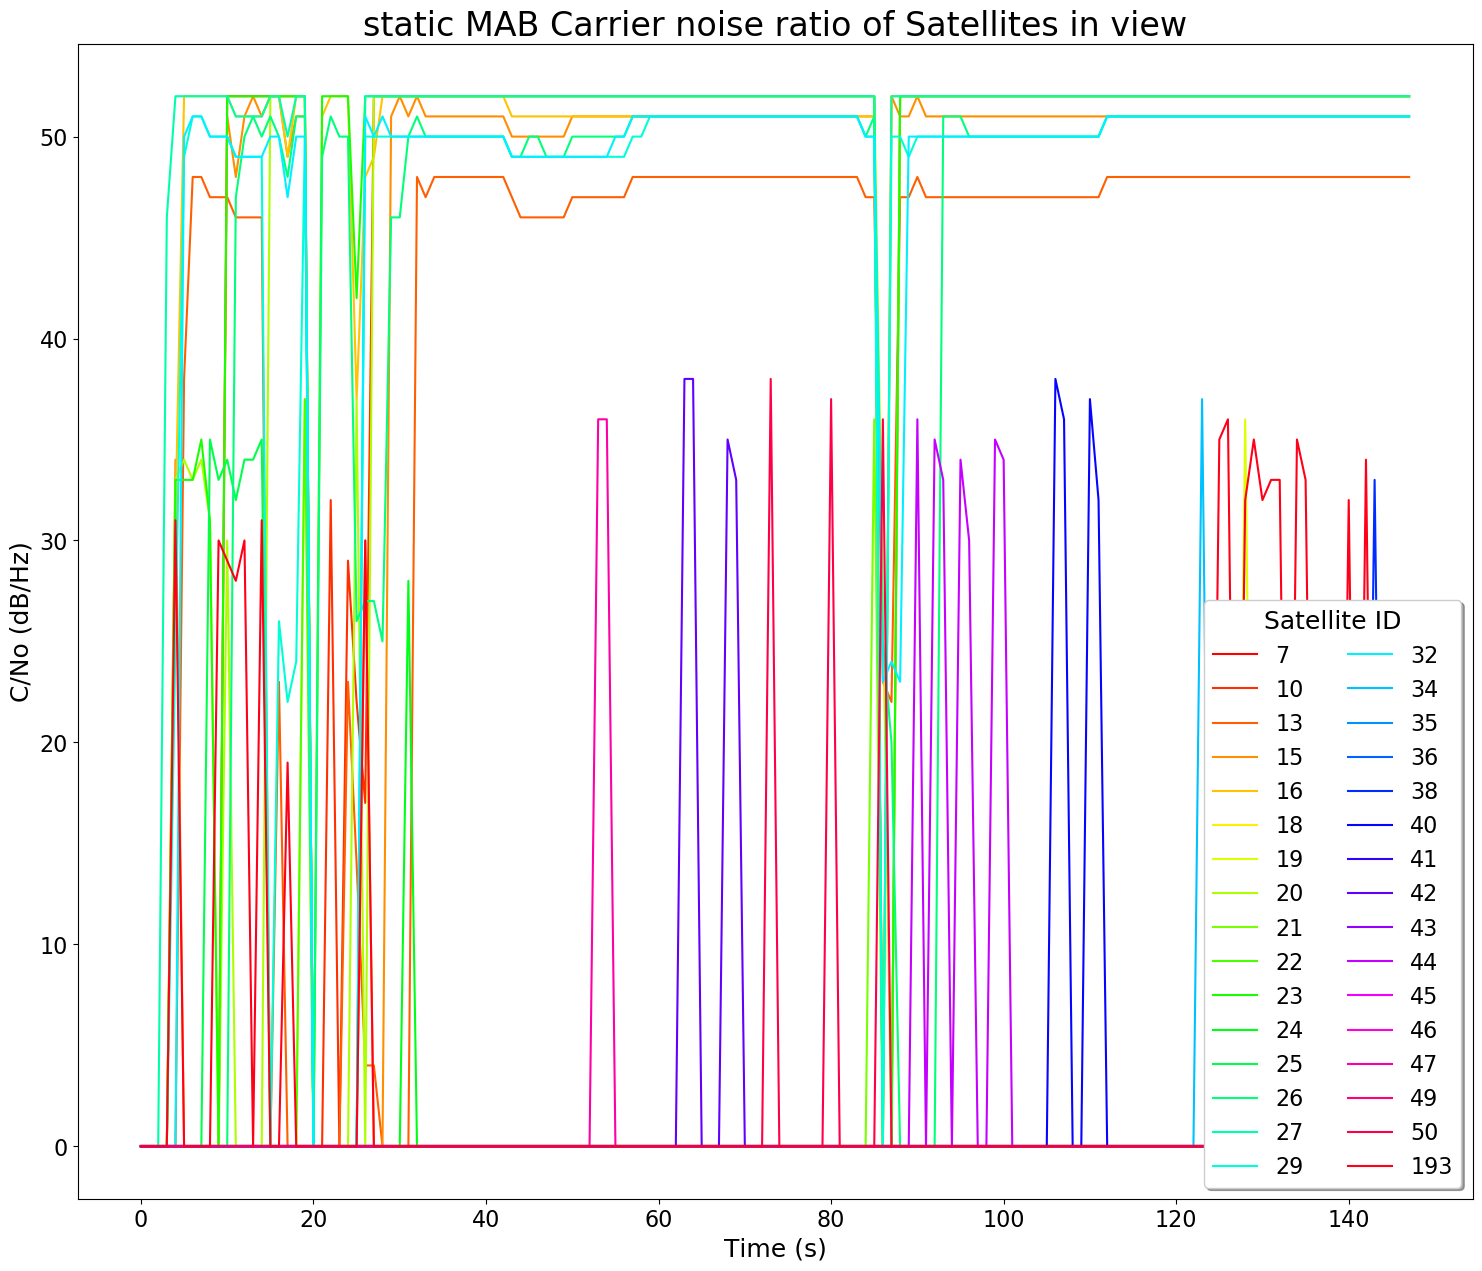
\includegraphics[width=12cm,keepaspectratio]{Figures/2021_3_30_static_MAB Carrier noise ratio.png}
        \caption{Carrier to noise ratio from unique SVIDs as broadcast by SDR and received by GPS receiver at MAB in Tonsley on 30th March 2021. Each SVID has been given a unique colour.}
        \label{fig:MABStaticCNo}
    \end{centering}
\end{figure}

From Figures \ref{fig:MABStaticCoord} and \ref{fig:MABStaticPosition} it can be seen that there are not many GPS location points on this graph, so while the spoof was
successful in the sense that the receiver was able to interpret a location and the calculated location had acceptable error values (<10m) there was clearly not a consistent lock. 

\begin{figure}[H]
    \begin{centering}
        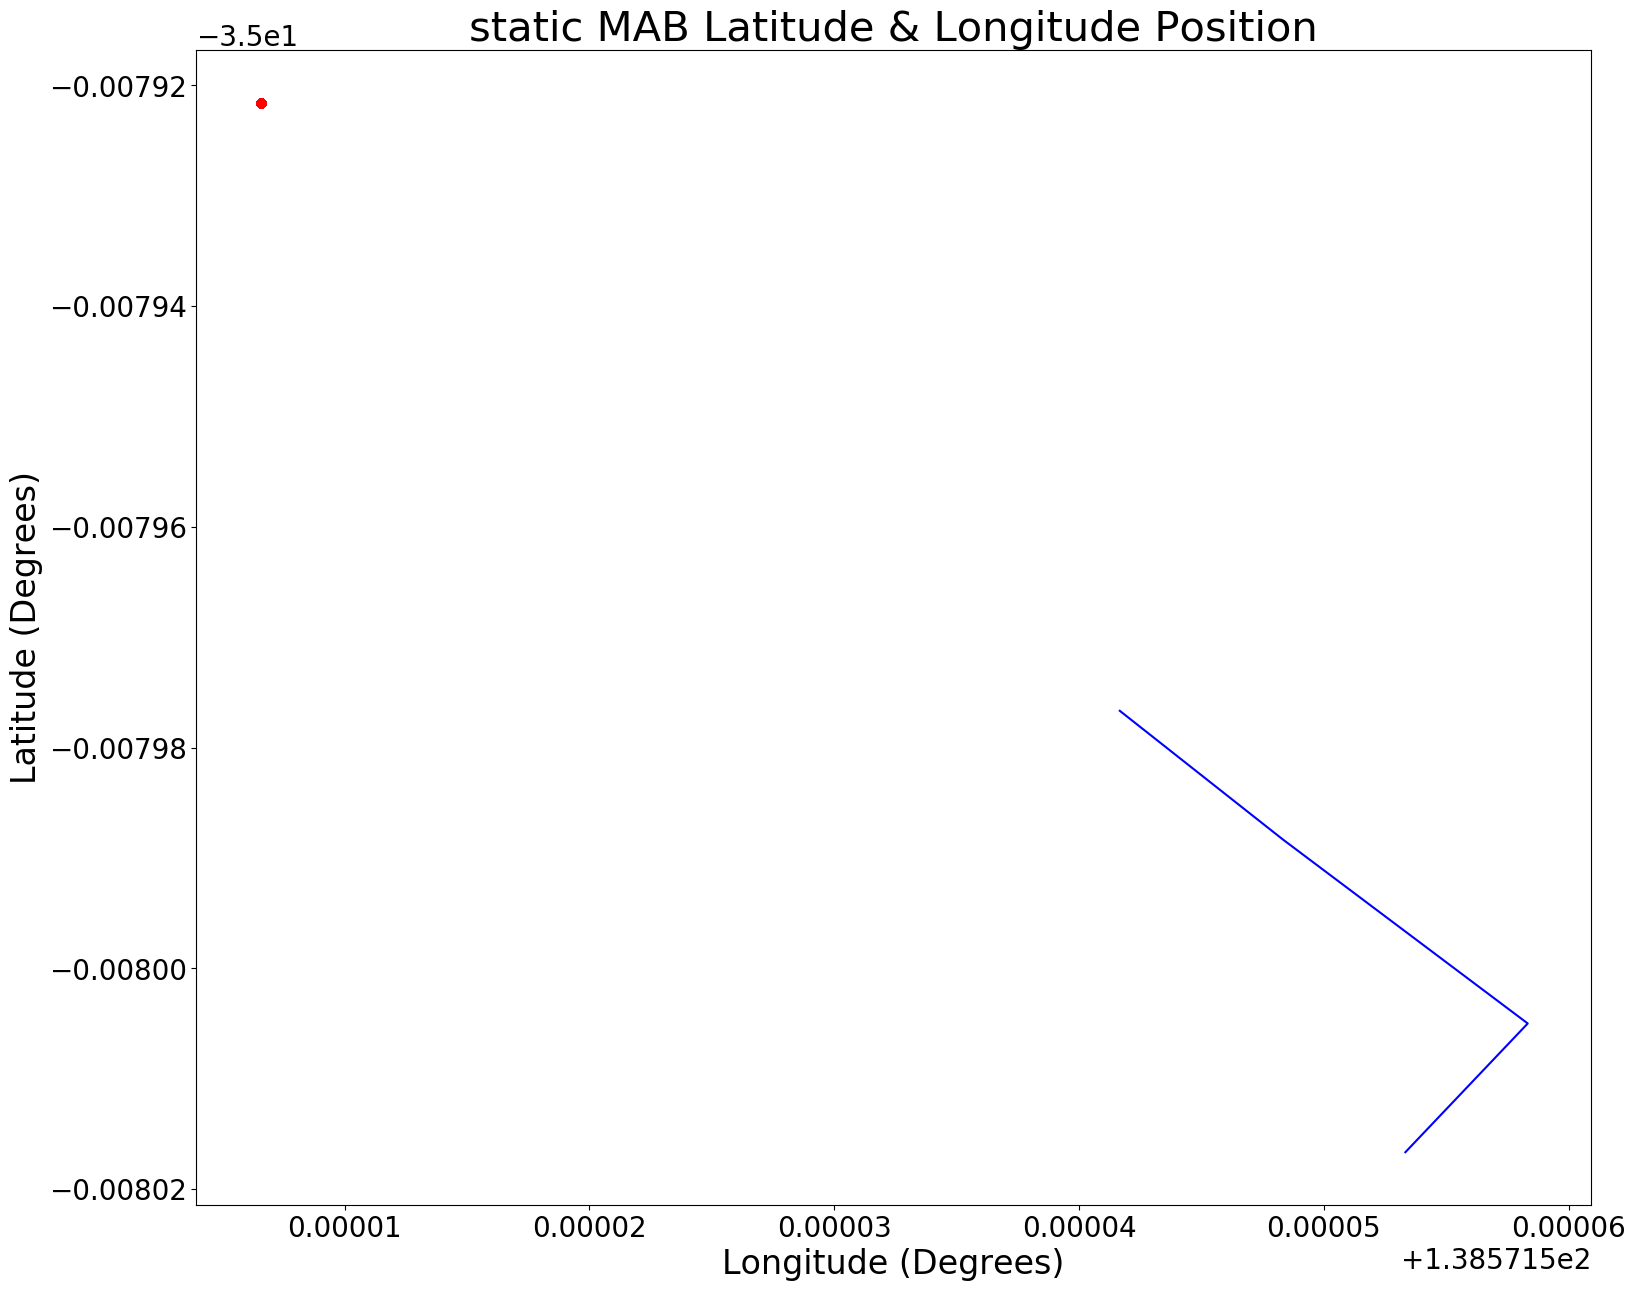
\includegraphics[width=12cm,keepaspectratio]{Figures/2021_3_30_static_MAB Lat long position.png}
        \caption{Trace of latitude and longitude over time as interpreted from the GPS receiver with expected location noted with red dot}
        \label{fig:MABStaticCoord}
    \end{centering}
\end{figure}

\begin{figure}[H]
    \begin{centering}
        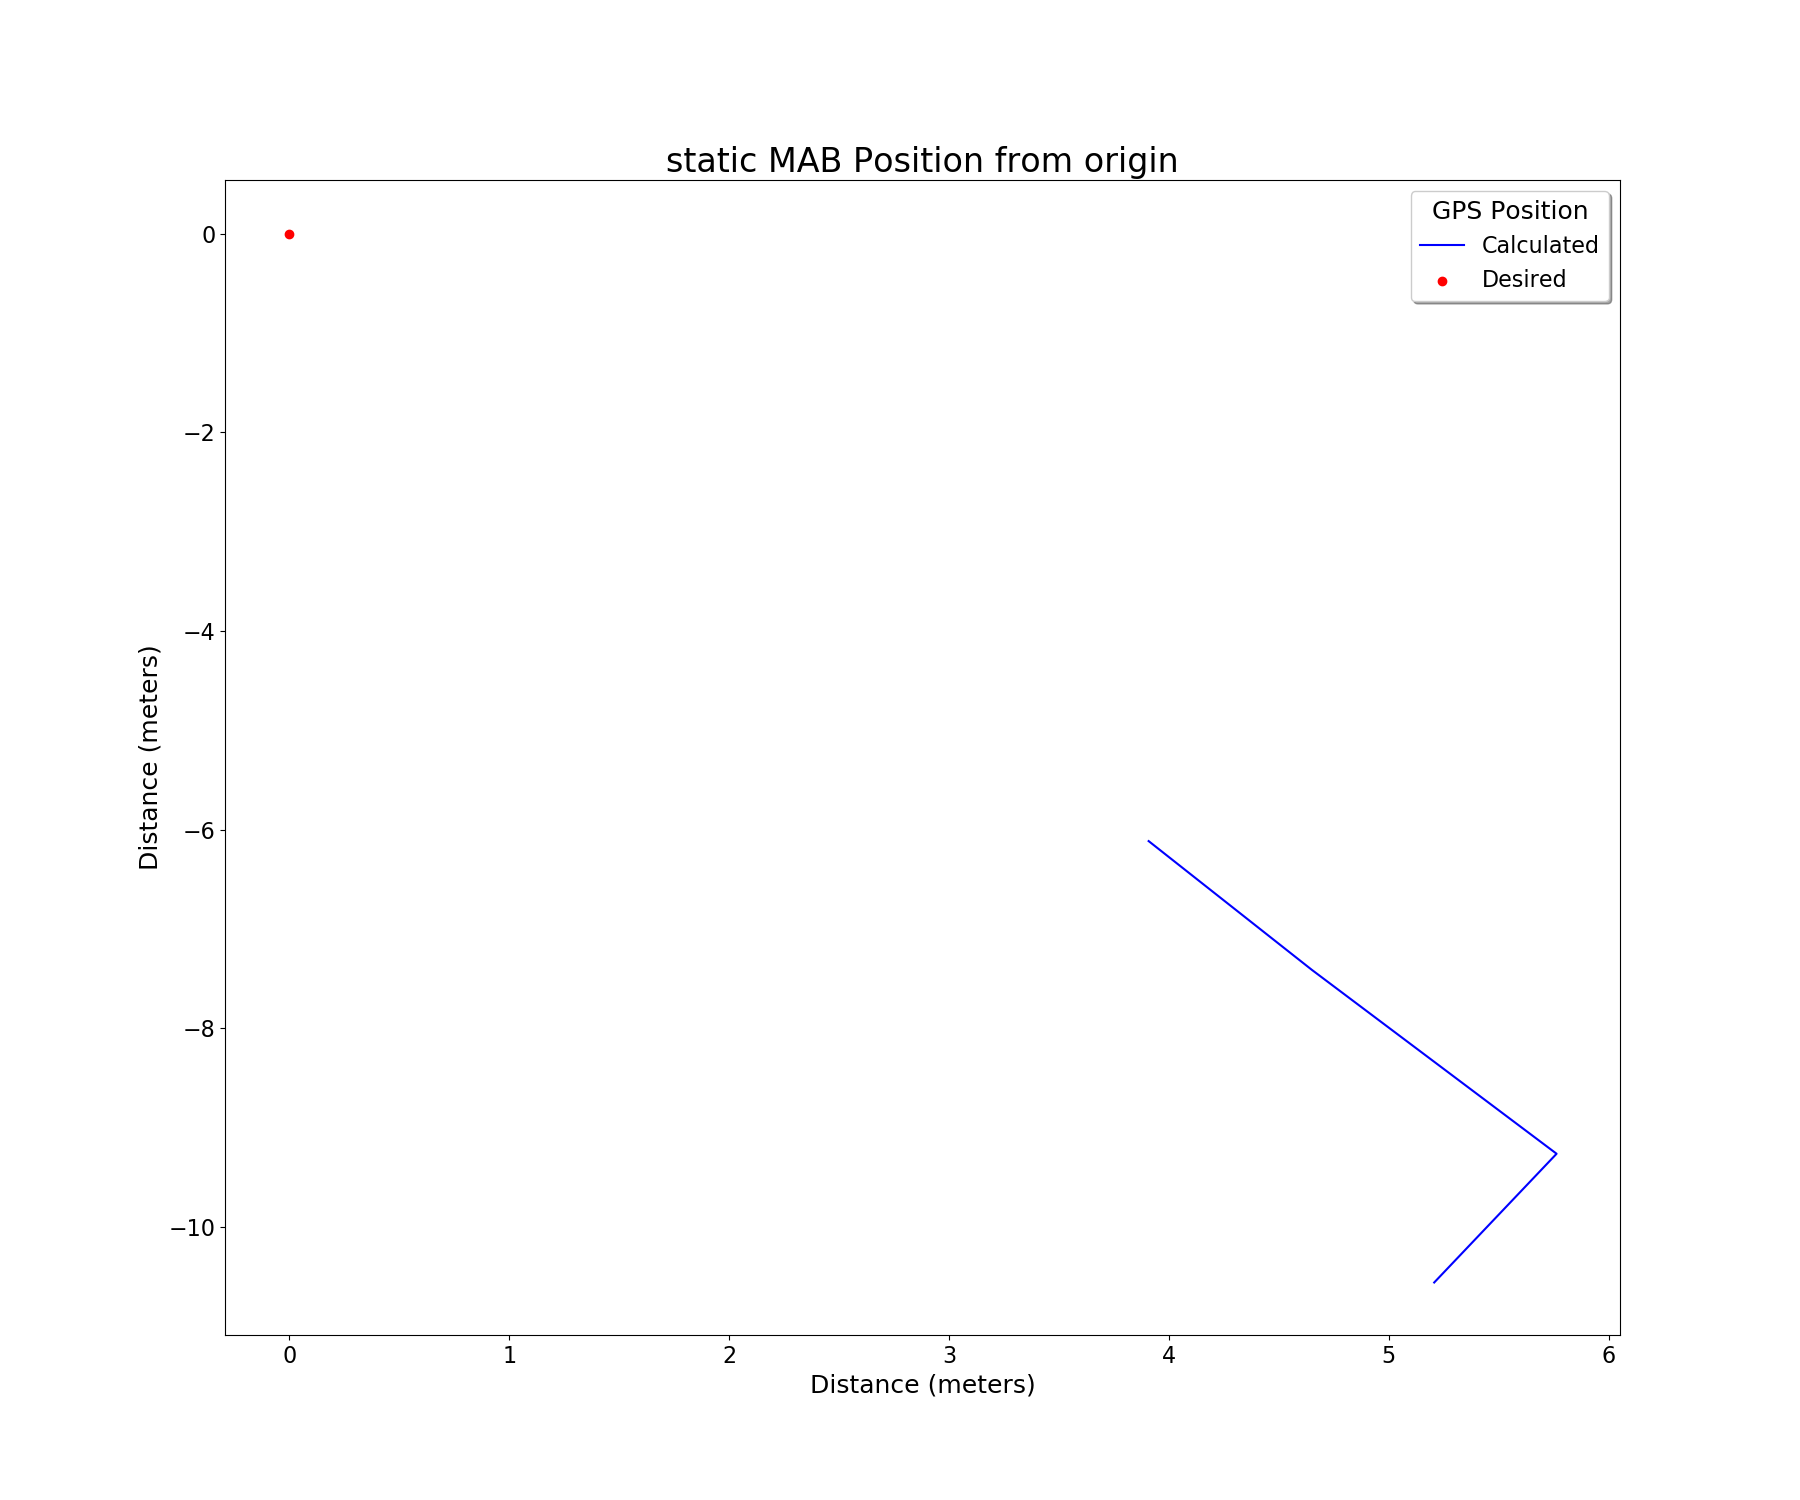
\includegraphics[width=12cm,keepaspectratio]{Figures/2021_3_30_static_MAB Position from origin.png}
        \caption{Graph of recorded position with respect to the intended spoofed location}
        \label{fig:MABStaticPosition}
    \end{centering}
\end{figure}

This
experiment should have been redone ensuring that there was no interference in the Faraday cage causing the lock to be lost. 
The extent of the error and lack of data points are more evident in Figures \ref{fig:MABStaticError} and \ref{fig:MABSatelliteImage}.

\begin{figure}[H]
    \begin{centering}
        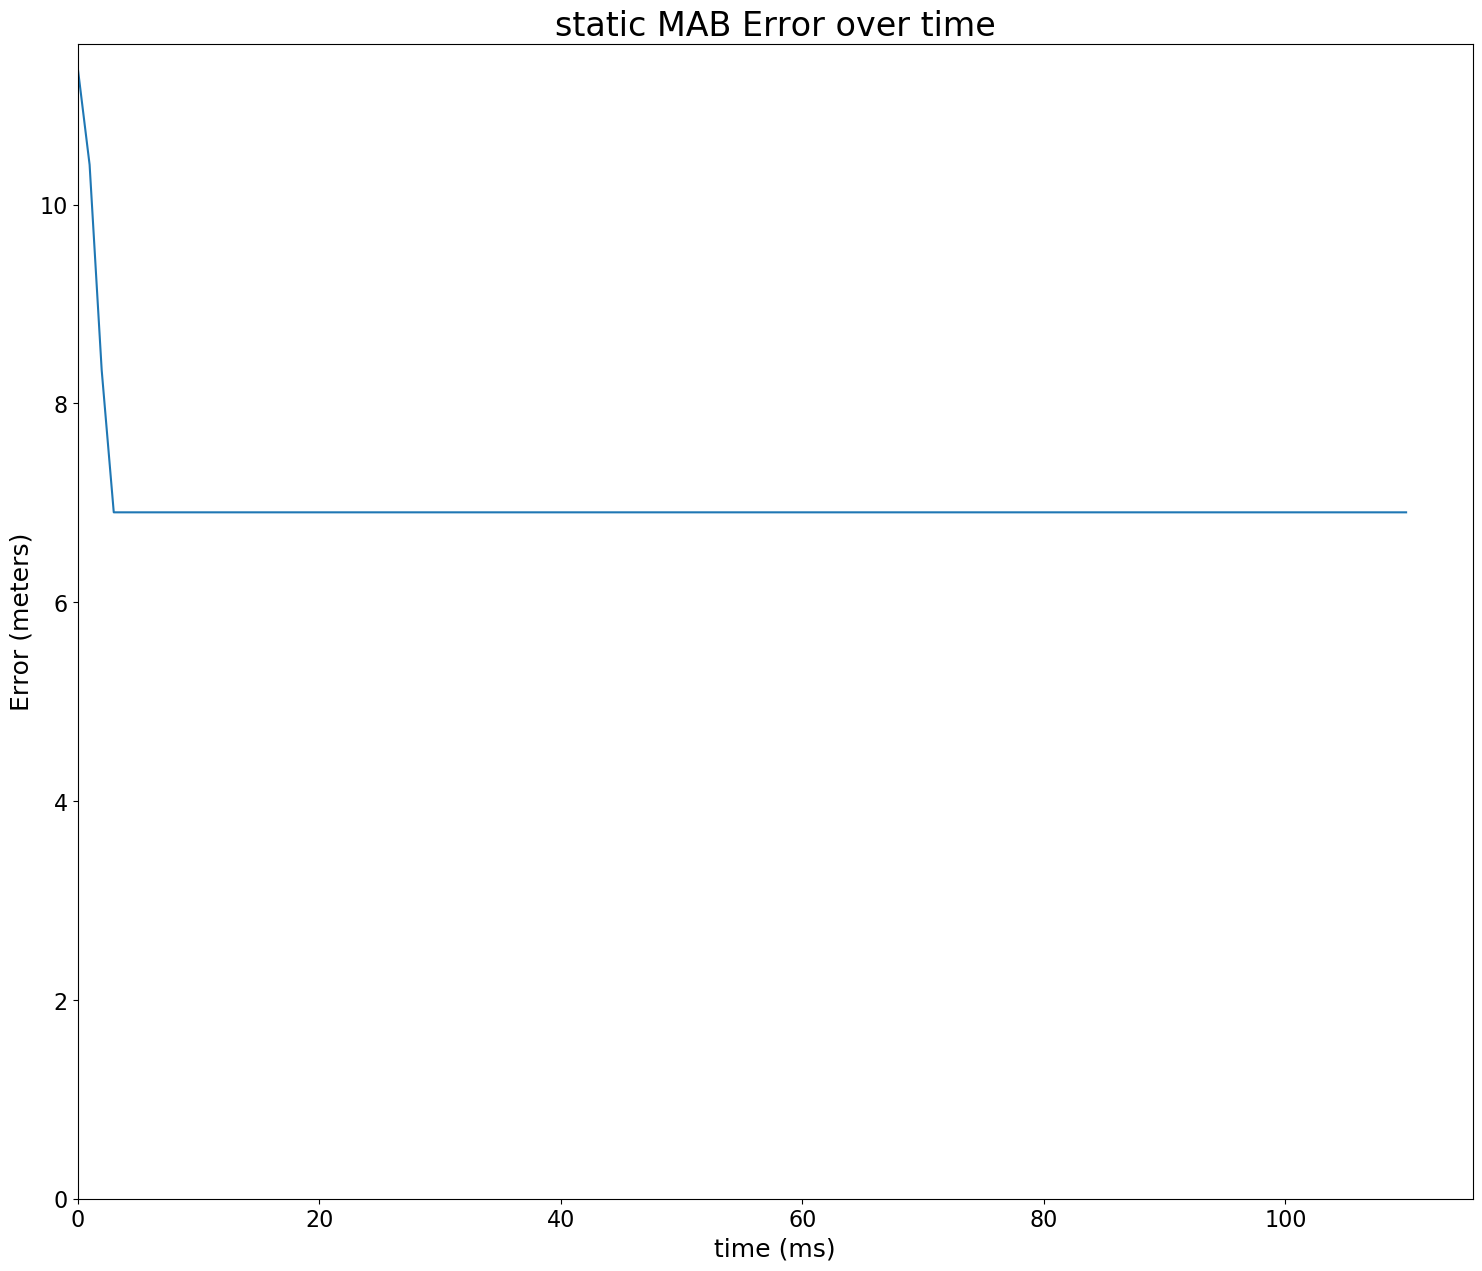
\includegraphics[width=12cm,keepaspectratio]{Figures/2021_3_30_static_MAB error over time.png}
        \caption{Error between calculated location and expected location over time}
        \label{fig:MABStaticError}
    \end{centering}
\end{figure}

\begin{figure}[H]
    \begin{centering}
        \includegraphics[width=12cm,keepaspectratio]{Figures/2021_3_30_static_MAB_Satellite.PNG}
        \caption{Satellite image of the MAB area next to Flinders University with expected GPS position shown with red cross and recorded position shown with blue line}
        \label{fig:MABSatelliteImage}
    \end{centering}
\end{figure}

\subsubsection{Antarctica}
Davis station in Antarctica was chosen as a location for spoofing. As mentioned above the coordinates for this location was $-68.5762449235, 77.9696166515$. The COTS
receiver was used as a spoof victim and it was successfully spoofed. Figure \ref{fig:antarcticaStaticCNo} shows the carrier to noise graph over the spoof attack. There is
a consistent value of $\approx 50 dBHz$ plus signals that are consistently at $\approx 40 dBHz$. These values indicate low interference and high signal quality. There
were more SVIDs (or PRN codes) than expected, with more SVIDs recorded than there are GPS satellites in operation. 
Time to first fix was shown to be approximately 60 seconds, this is the lower end of the fix times from experiments for cold starts. 
It can be see that there is consistent signals for the first 50 seconds. For the time period between 70 and
200 seconds there was more volatile signal quality. 

\begin{figure}[H]
    \begin{centering}
        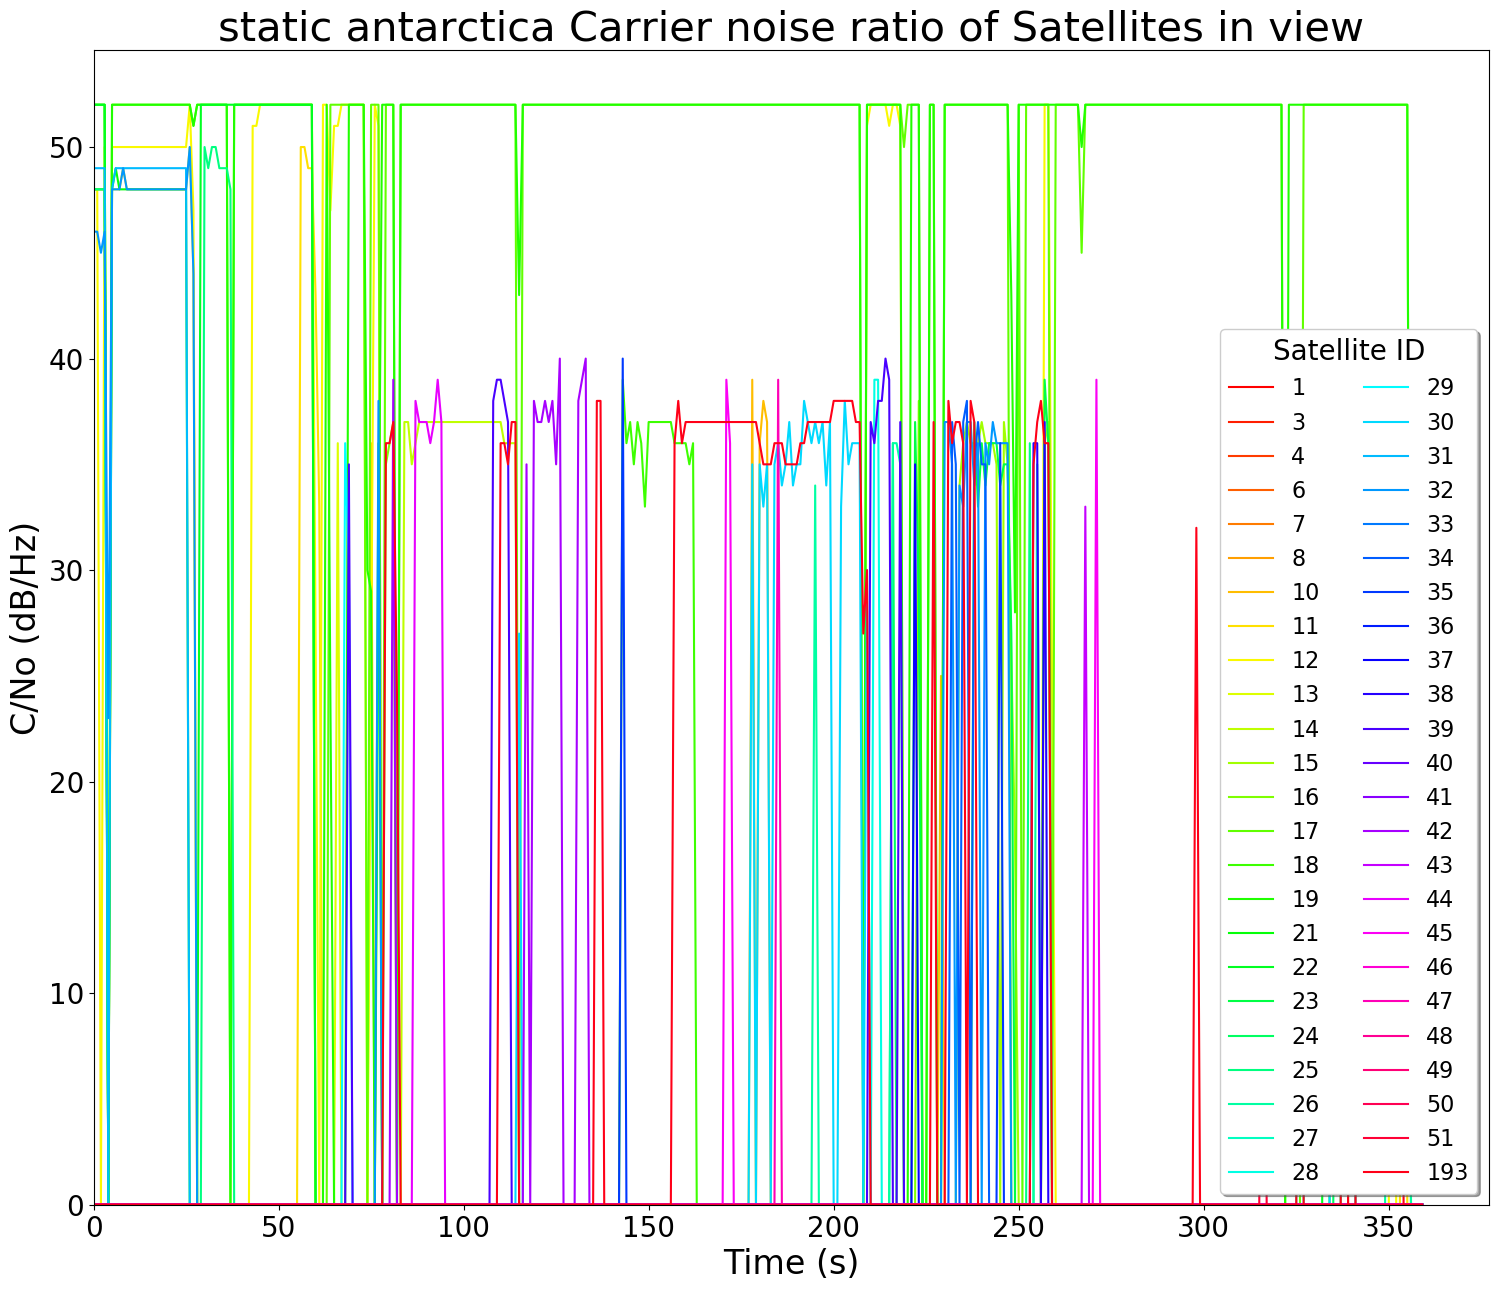
\includegraphics[width=12cm,keepaspectratio]{Figures/2021_3_30_static_antarctica Carrier noise ratio.png}
        \caption{Carrier to noise ratio from unique SVIDs as broadcast by SDR and received by GPS receiver at Davis Station in Antarctica on 30th March 2021. Each SVID has been given a unique colour.}
        \label{fig:antarcticaStaticCNo}
    \end{centering}
\end{figure}

Figure \ref{fig:antarcticaStaticError} shows that there was a high, but consistent level of error between first fix
and 140 seconds. After this there was a spike, which is associated with a drop of lock, and the high error remained until the end of the test. This may have been due to
the satellite geometry and DOP values. Receivers at the poles are prone to higher DOP values \cite{RN62}. This high error is evident
when viewing the raw position in Figure \ref{fig:antarcticaStaticCoord} and with respect to the desired location, Figure \ref{fig:antarcticaStaticPosition}. Figure \ref{fig:antarcticaSatelliteImage} shows this error
in position in more context placed over a satellite image.
The inaccuracy is higher than was expected from this experiment.  

\begin{figure}[H]
    \begin{centering}
        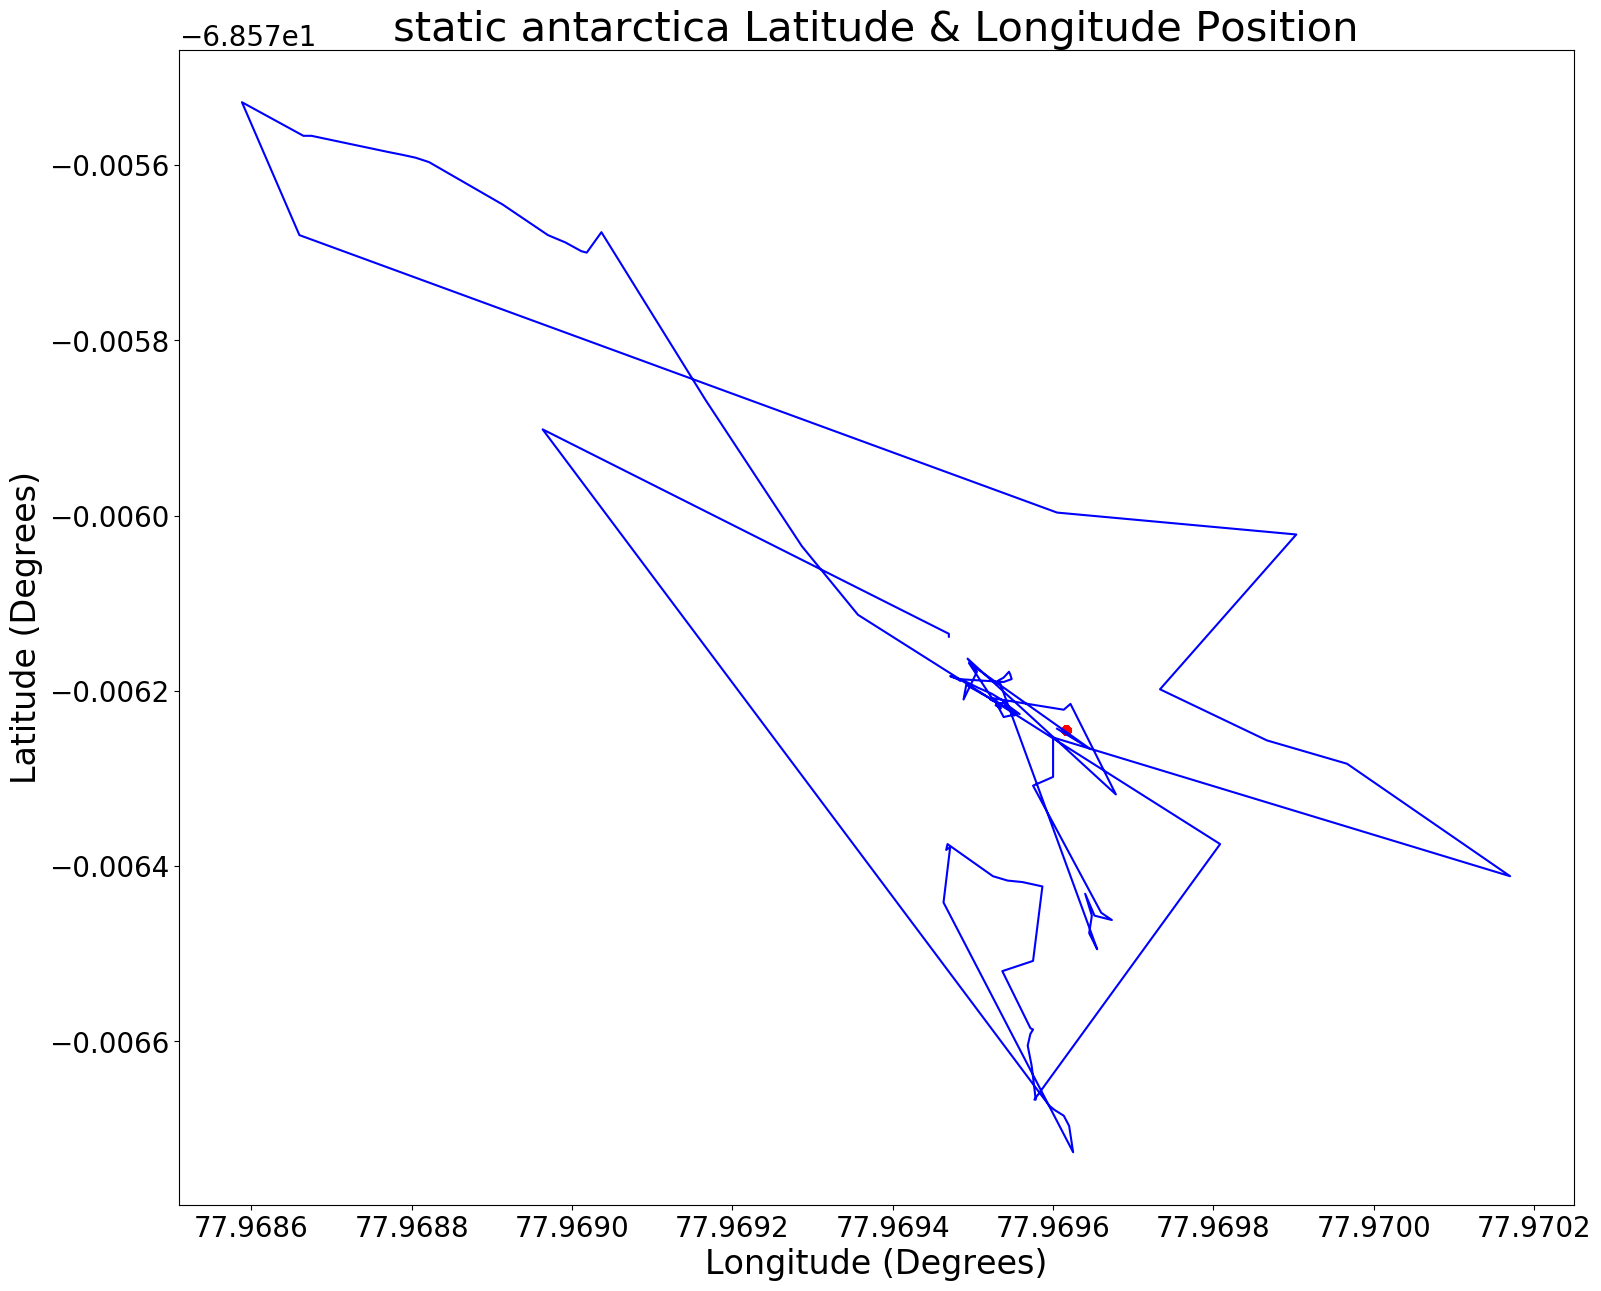
\includegraphics[width=12cm,keepaspectratio]{Figures/2021_3_30_static_antarctica Lat long position.png}
        \caption{Trace of latitude and longitude over time as interpreted from the GPS receiver with expected location noted with red dot}
        \label{fig:antarcticaStaticCoord}
    \end{centering}
\end{figure}

\begin{figure}[H]
    \begin{centering}
        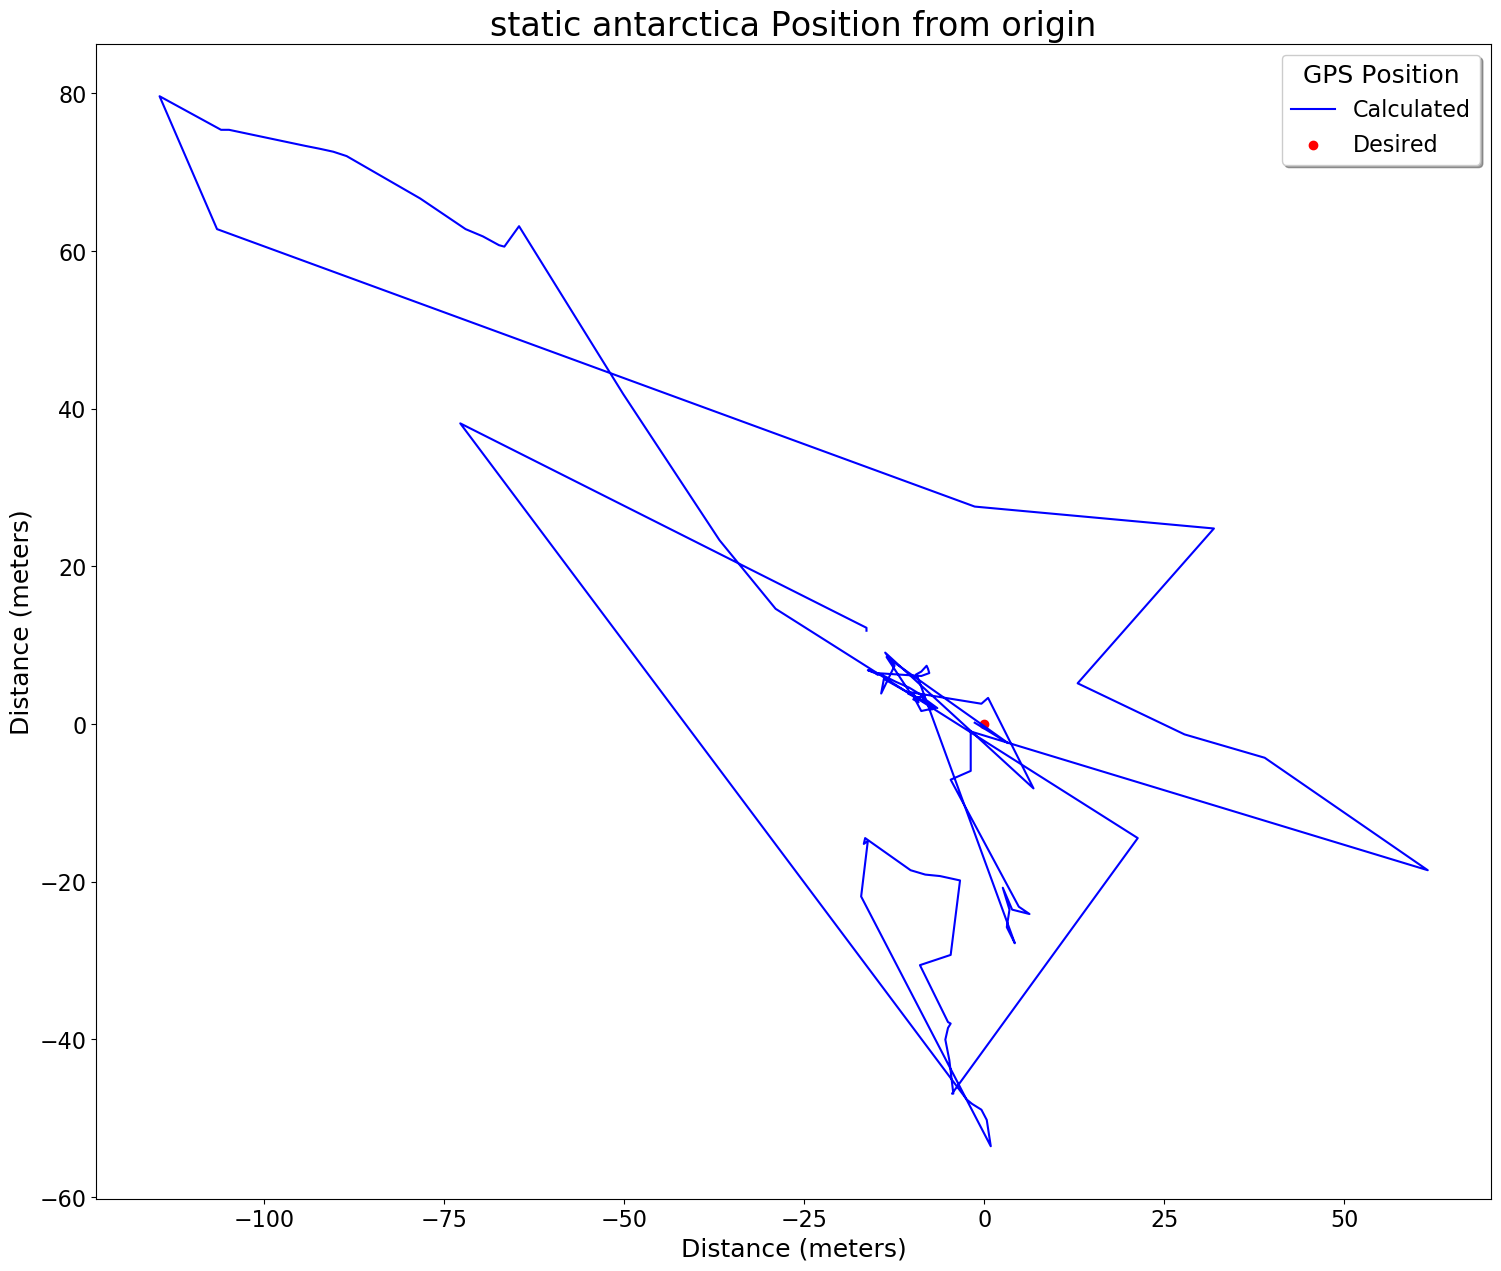
\includegraphics[width=12cm,keepaspectratio]{Figures/2021_3_30_static_antarctica Position from origin.png}
        \caption{Graph of recorded position with respect to the intended spoofed location}
        \label{fig:antarcticaStaticPosition}
    \end{centering}
\end{figure}

\begin{figure}[H]
    \begin{centering}
        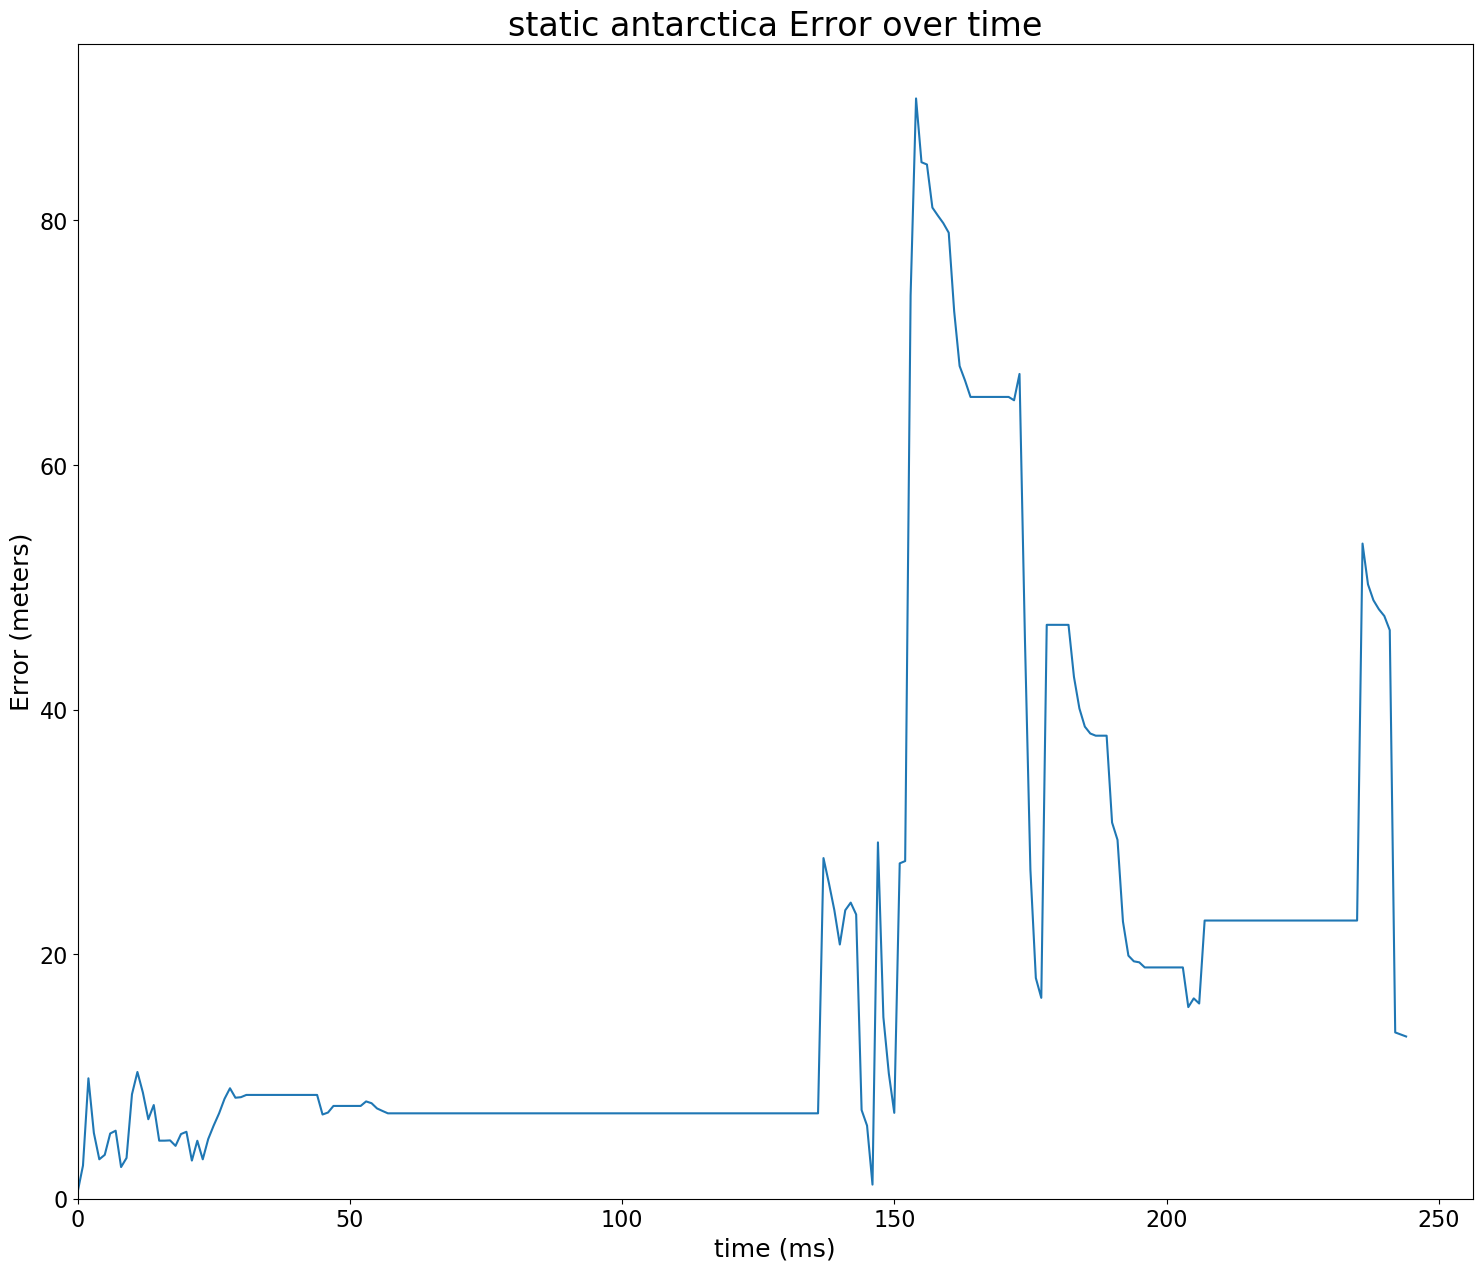
\includegraphics[width=12cm,keepaspectratio]{Figures/2021_3_30_static_antarctica error over time.png}
        \caption{Error between calculated location and expected location over time}
        \label{fig:antarcticaStaticError}
    \end{centering}
\end{figure}

\begin{figure}[H]
    \begin{centering}
        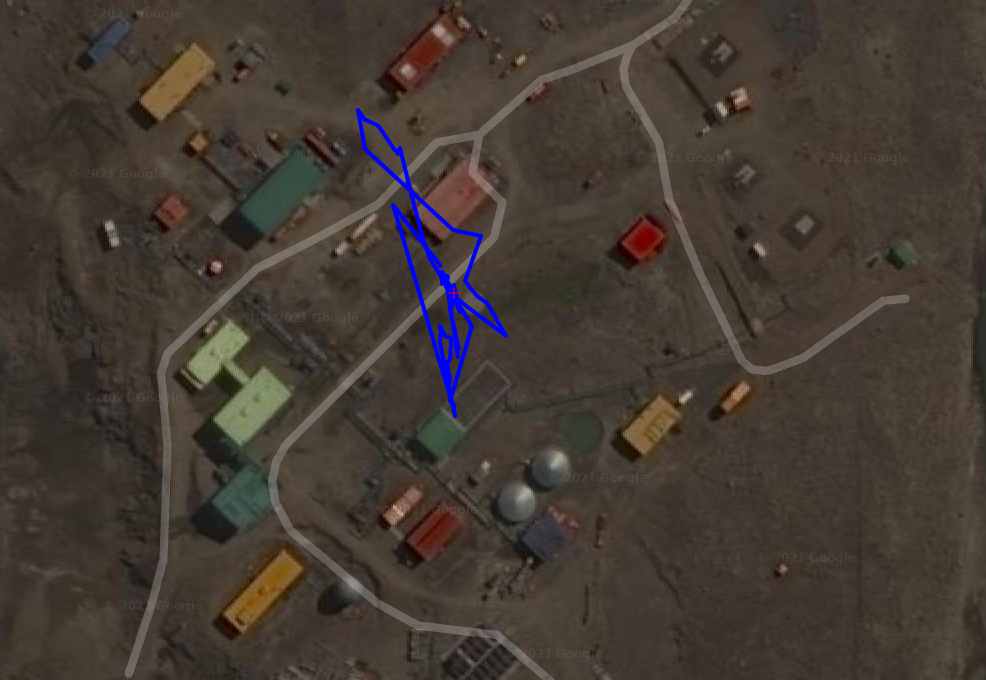
\includegraphics[width=12cm,keepaspectratio]{Figures/2021_3_30_static_antarctica_Satellite.PNG}
        \caption{Satellite image with expected GPS position shown with red cross and recorded position shown with blue line}
        \label{fig:antarcticaSatelliteImage}
    \end{centering}
\end{figure}

\subsection{Dynamic Spoofing}
Dynamic spoofing attacks were also performed. These attacks do not have a set coordinate that the spoofer is attempting to make the receiver appear at, rather these
attacks try to get the receiver to "follow" a path that has been set, see Section \ref{subsec:coordinate}.
\subsubsection{Tonsley MAB}
There is a road that circles around the MAB (Mass Assembly Building) in which the \univname Tonsley campus is situated. This was used as a path to spoof the GPS receiver,
see Figure \ref{fig:MABdynamicSetup}.

\begin{figure}[H]
    \begin{centering}
        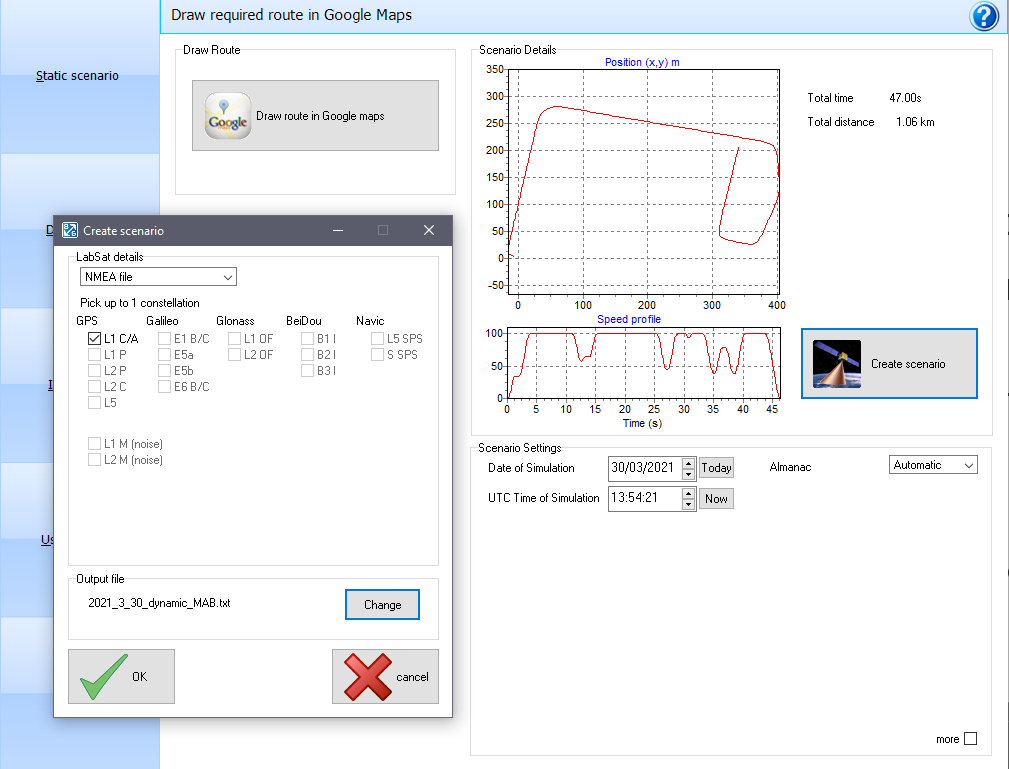
\includegraphics[width=14cm,keepaspectratio]{Figures/2021_3_30_dynamic_MAB_setup.png}
        \caption{Using road around the MAB at Tonsley, Adelaide as path for dynamic spoofing attack. The file was saved as a text file to be compiled into a binary.}
        \label{fig:MABdynamicSetup}
    \end{centering}
\end{figure}

The time to first fix was found to be approximately 49 seconds which is considered quick for a cold start. The $\frac{C}{N_0}$ ratio graph, see \ref{fig:MABdynamicCNo} shows a common trend of having
a high average of $\approx 50dBHz$ average with some lower values from spikes. These spikes would not add any value to the quality of the fix and given more time the
cause of the spikes would be found. From Figure \ref{fig:MABdynamicCoord} it can be seen that initially there was high amounts of error while getting the initial fix.
Though when the movement began there was good tracking. This is evident in Figure \ref{fig:MABdynamicPosition} where the reference path and received path were overlaid.
Overlaying onto a satellite image yielded figure \ref{fig:MABdynamicSatelliteImage} which shows how well the spoof attack was able to track the reference path. This produced
results that would be expected from authentic GPS signals, with the exception being the initial part of the experiment. 

\begin{figure}[H]
    \begin{centering}
        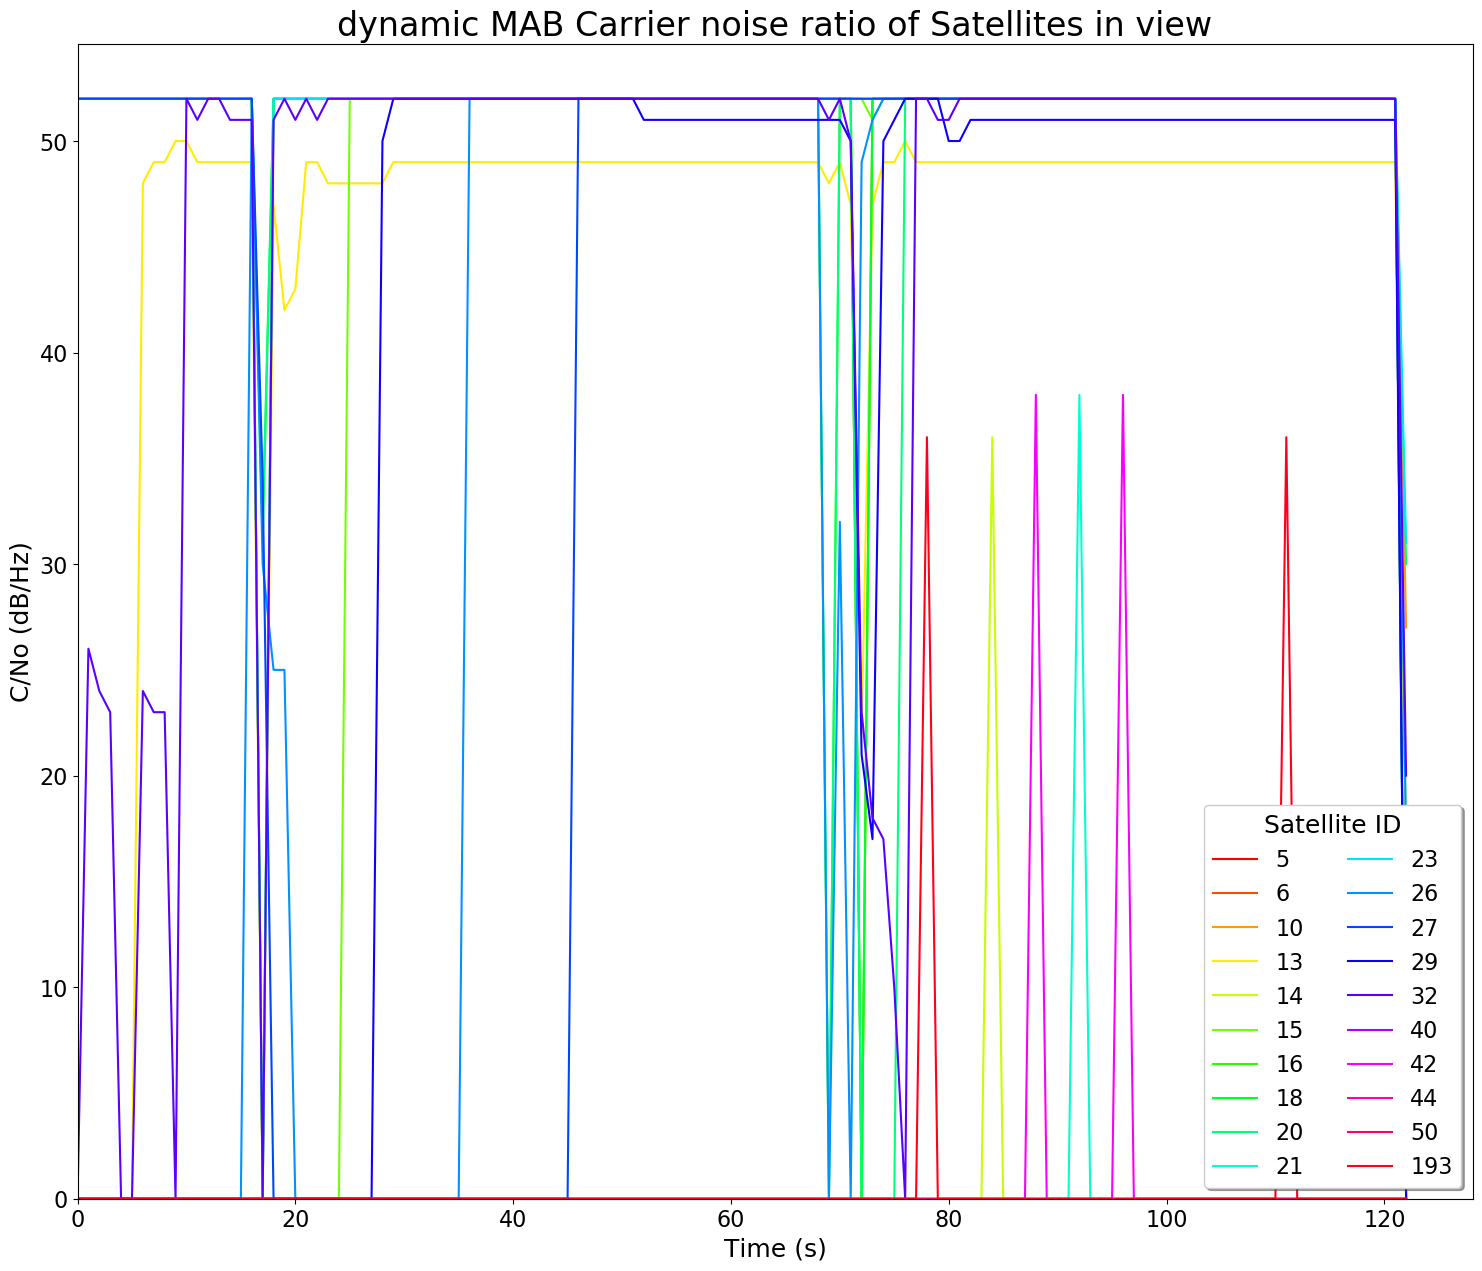
\includegraphics[width=12cm,keepaspectratio]{Figures/2021_3_30_dynamic_MAB Carrier noise ratio.png}
        \caption{Carrier to noise ratio from unique SVIDs as broadcast by SDR and received by GPS receiver at MAB in Tonsley on 30th March 2021. Each SVID has been given a unique colour.}
        \label{fig:MABdynamicCNo}
    \end{centering}
\end{figure}

\begin{figure}[H]
    \begin{centering}
        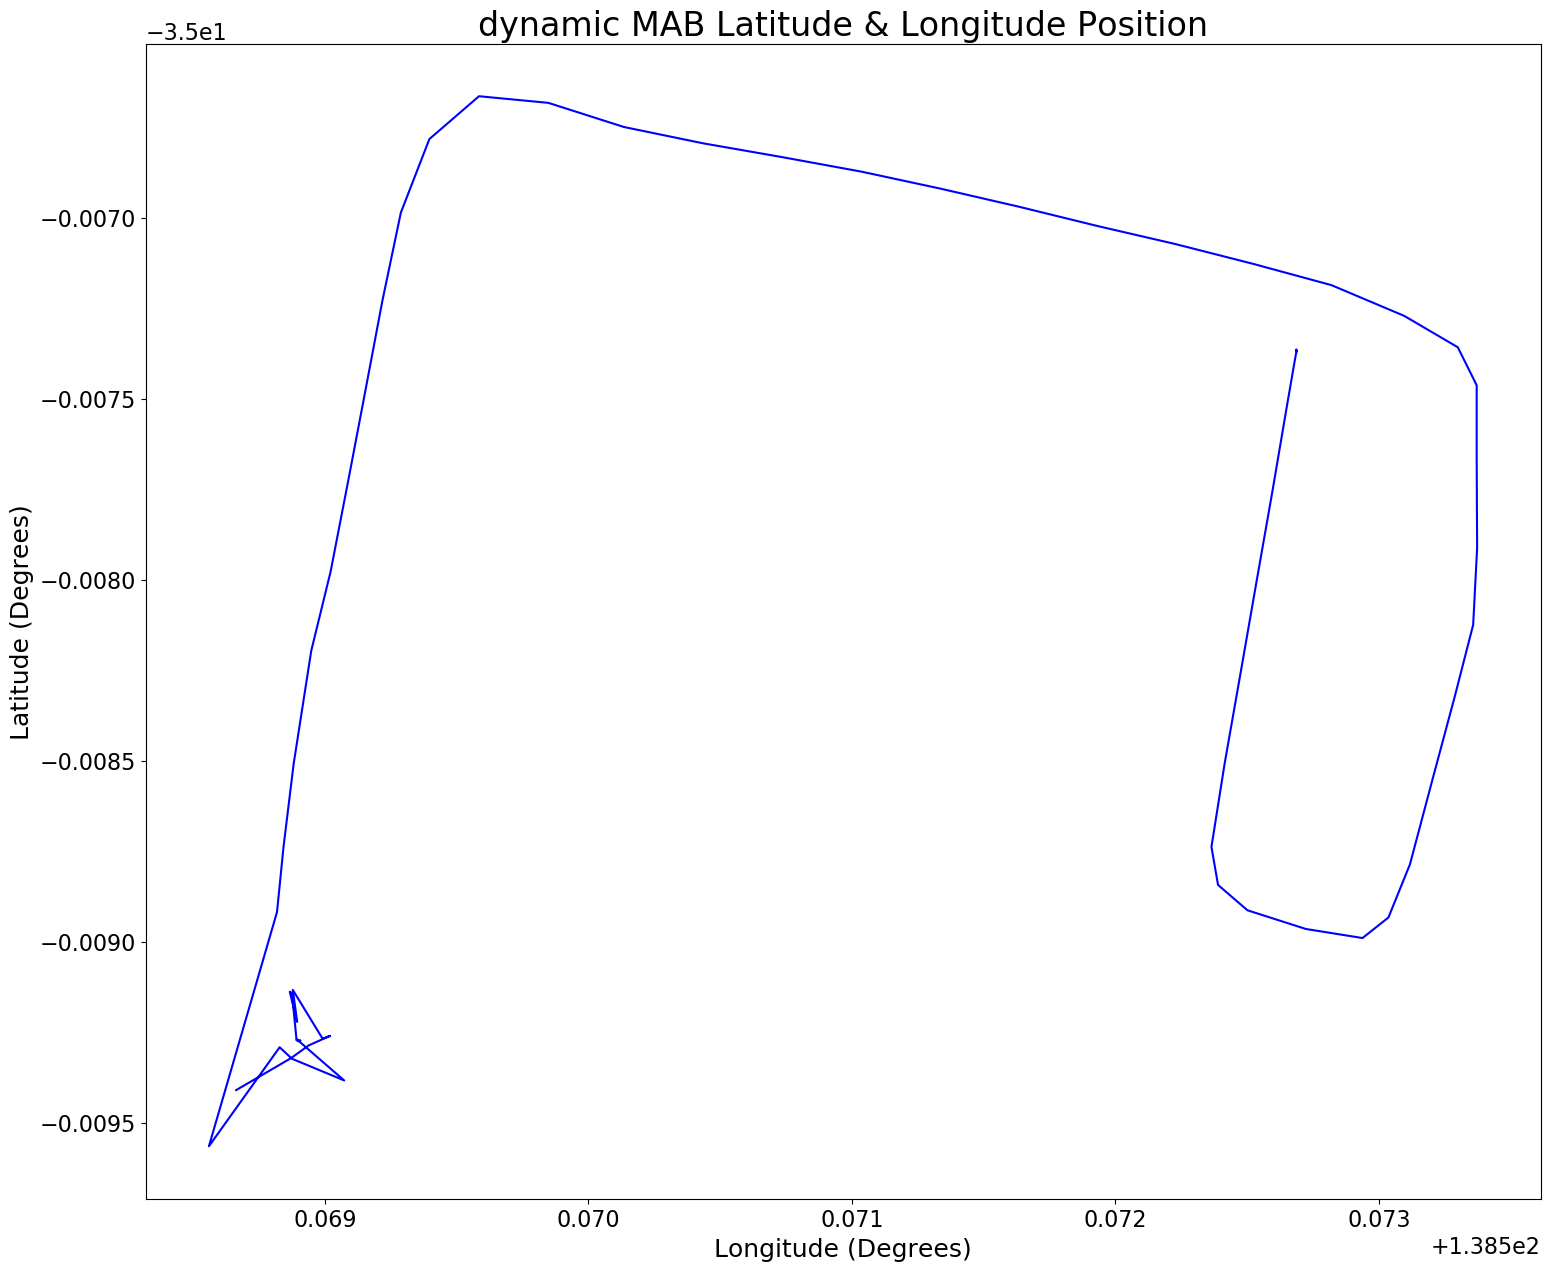
\includegraphics[width=12cm,keepaspectratio]{Figures/2021_3_30_dynamic_MAB Lat long position.png}
        \caption{Trace of latitude and longitude over time as interpreted from the GPS receiver}
        \label{fig:MABdynamicCoord}
    \end{centering}
\end{figure}

\begin{figure}[H]
    \begin{centering}
        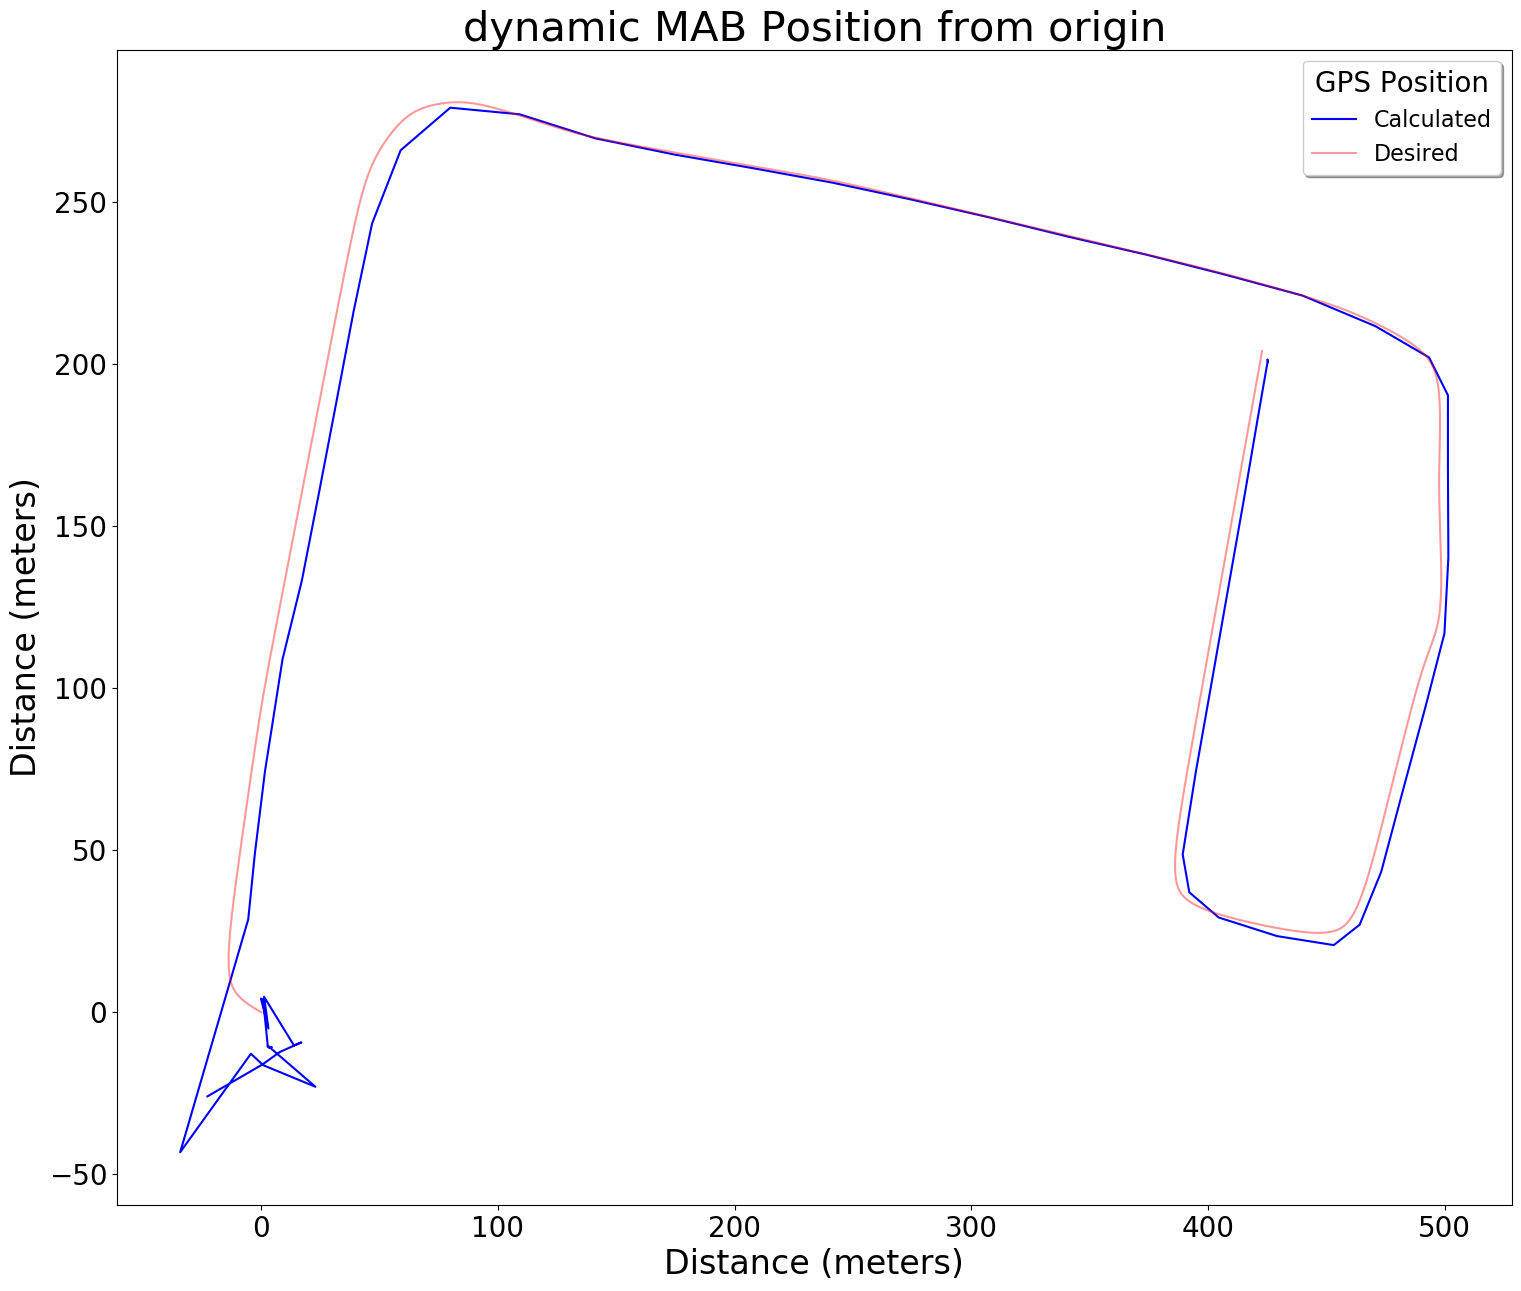
\includegraphics[width=12cm,keepaspectratio]{Figures/2021_3_30_dynamic_MAB Position from origin.png}
        \caption{Graph of recorded position with respect to the reference location shown as a red path}
        \label{fig:MABdynamicPosition}
    \end{centering}
\end{figure}

\begin{figure}[H]
    \begin{centering}
        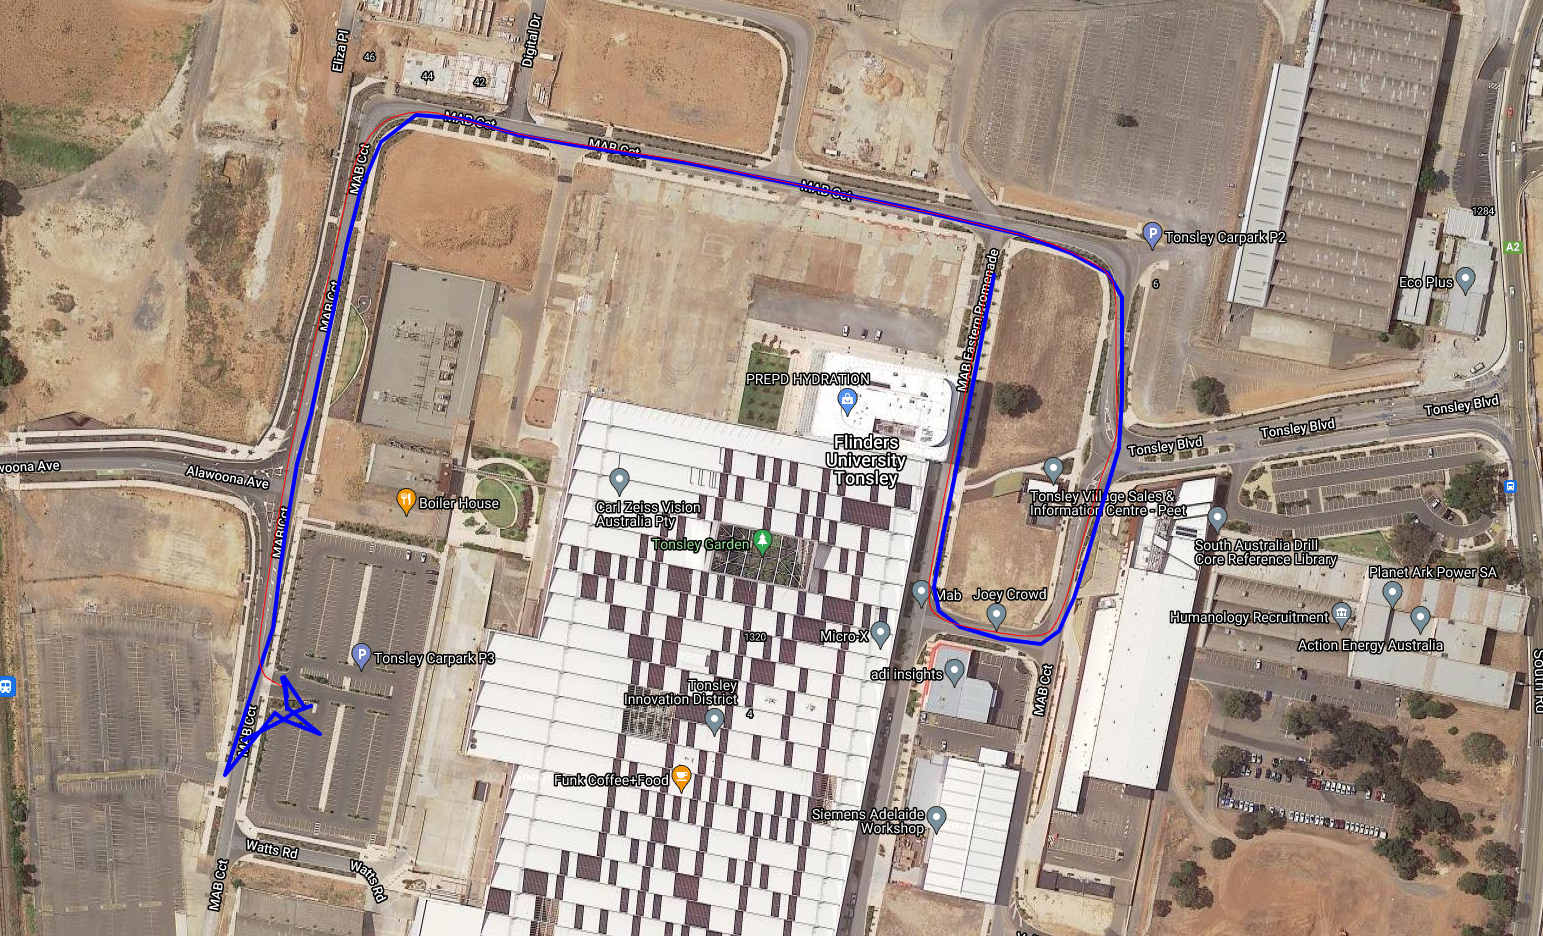
\includegraphics[width=14cm,keepaspectratio]{Figures/2021_3_30_dynamic_MAB_Satellite.PNG}
        \caption{Satellite image with expected GPS position shown with red cross and recorded position shown with blue line}
        \label{fig:MABdynamicSatelliteImage}
    \end{centering}
\end{figure}

\subsubsection{Adelaide CBD Loop}
After successfully performing a dynamic spoof attack around the MAB, a longer path was chosen to test how if the SDR was capable of sustaining spoofing performance for a
longer period of time. An abitrary path around the Adelaide CBD was chosen from within the SatGen3 software. As shown in figure \ref{fig:CBDdynamicSetup} the total time of the path was 643 seconds. This represents the total time of the spoofing transmission.

\begin{figure}[!h]
    \begin{centering}
        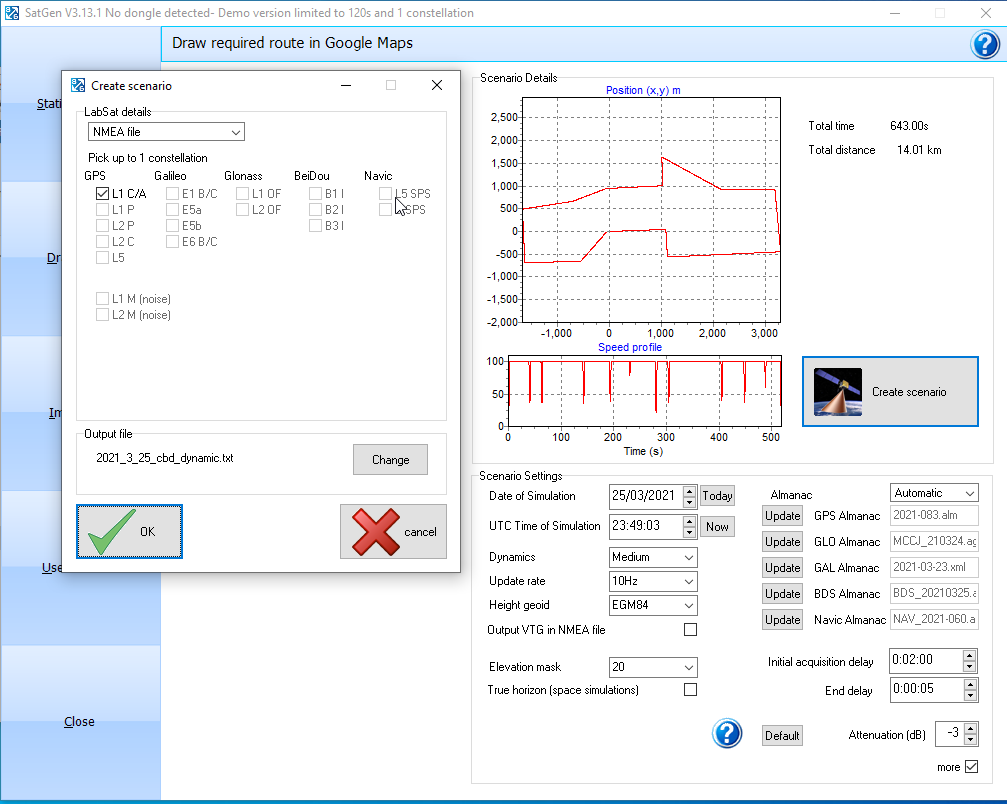
\includegraphics[width=12cm,keepaspectratio]{Figures/21-3-25_cbd_dynamic_longloop_setup.png}
        \caption{An arbitrary path was draw around the Adelaide CBD for dynamic spoofing attack. The file was saved as a text file to be compiled into a binary.}
        \label{fig:CBDdynamicSetup}
    \end{centering}
\end{figure}

The time to first fix for this test was 40 seconds. As previously mentioned this is considered a good result for a GPS receiver from a cold start. From figure
\ref{fig:CBDdynamicCNo} it can be seen that there was no unden run errors during the running of this test. Ther was a consistent few signals with $\frac{C}{N_0}$ values
of $>50dBHz$ with periodic other signals spiking at $\approx 40dBHz$.
The consistent issue of more SVIDs than satellite in the GPS constellation was present again in these results.

\begin{figure}[H]
    \begin{centering}
        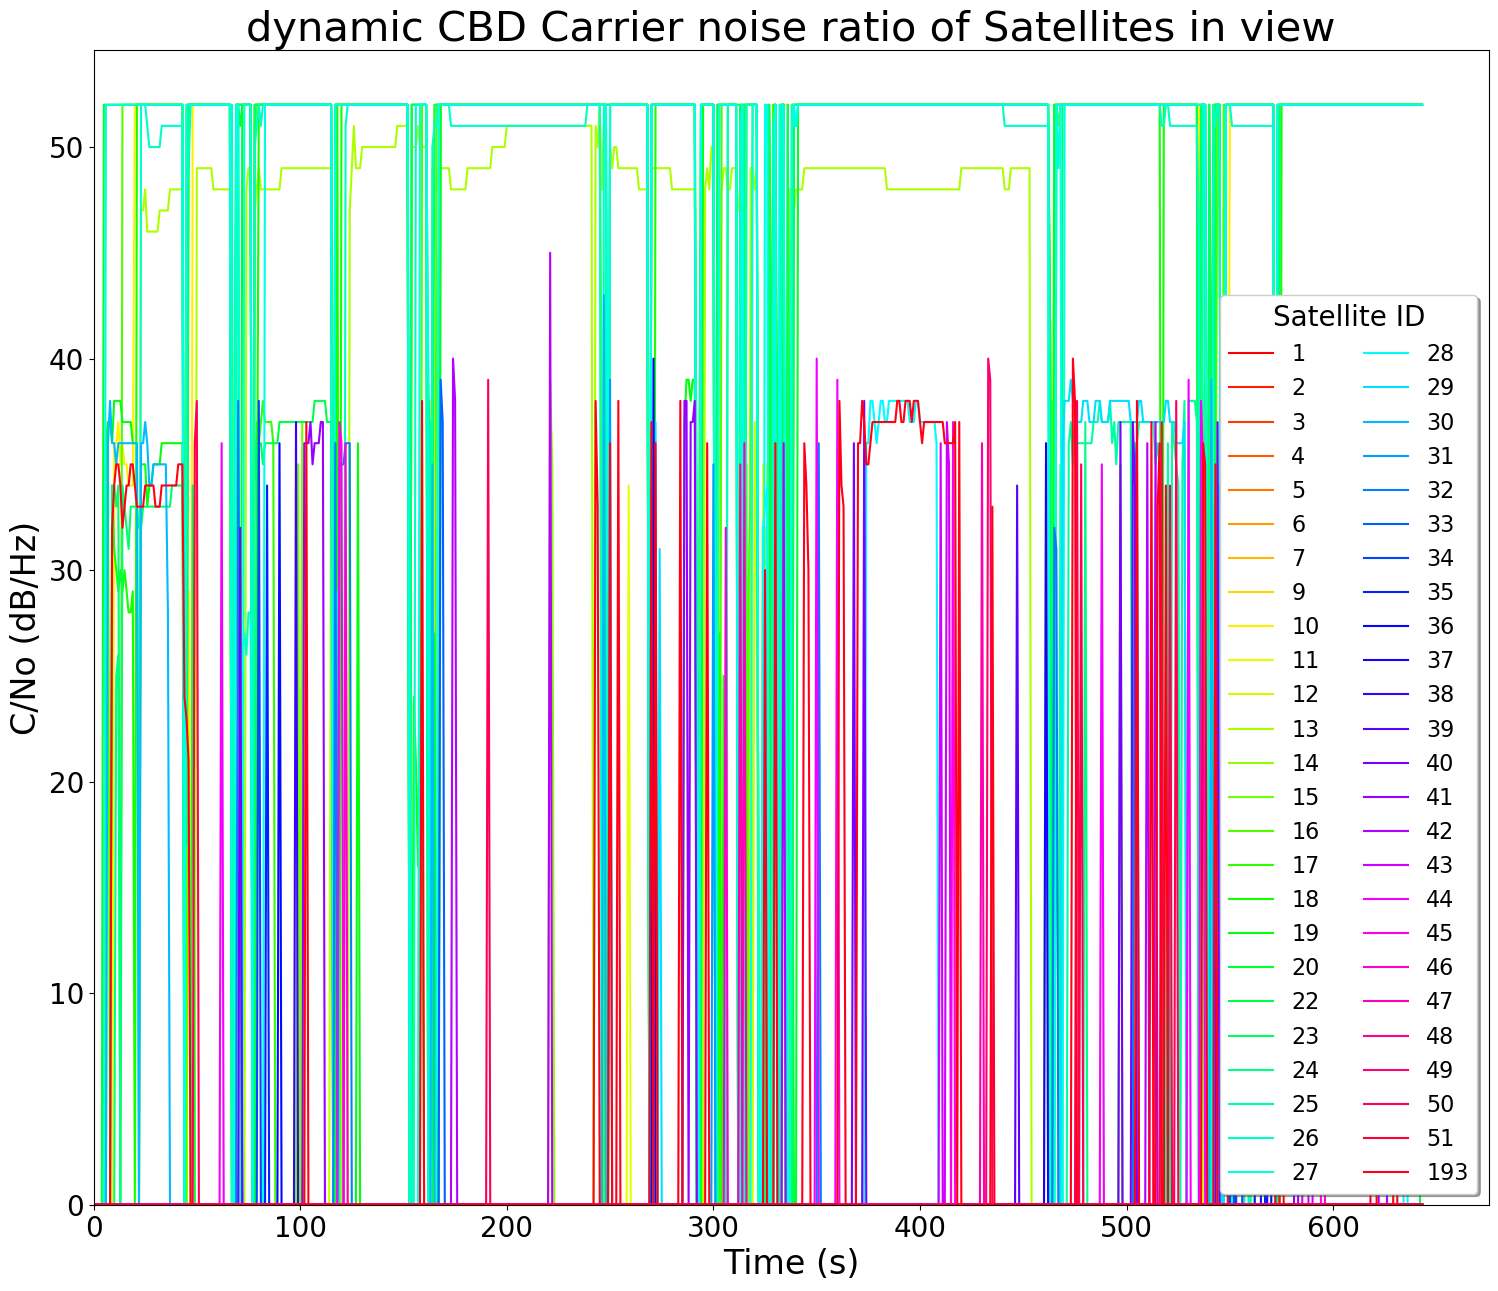
\includegraphics[width=12cm,keepaspectratio]{Figures/21_3_30_dynamic_CBD_results Carrier noise ratio.png}
        \caption{Carrier to noise ratio from unique SVIDs as broadcast by SDR and received by GPS receiver at Adelaide CBD on 30th March 2021. Each SVID has been given a unique colour.}
        \label{fig:CBDdynamicCNo}
    \end{centering}
\end{figure}

From figures \ref{fig:CBDdynamicCoord} and \ref{fig:CBDdynamicPosition} it can be seen that there was some error at the beginning of the test, shown as the (0,0) origin
in figure \ref{fig:CBDdynamicPosition}, but this smooths out as the test continued. There was more error introduced at various times during the rest of the test, but
overall the result was successul. Figure \ref{fig:CBDdynamicSatelliteImage} shows the context of the error over a satellite image. From this image it can be seen that the
extent of the error is typically acceptable.

\begin{figure}[H]
    \begin{centering}
        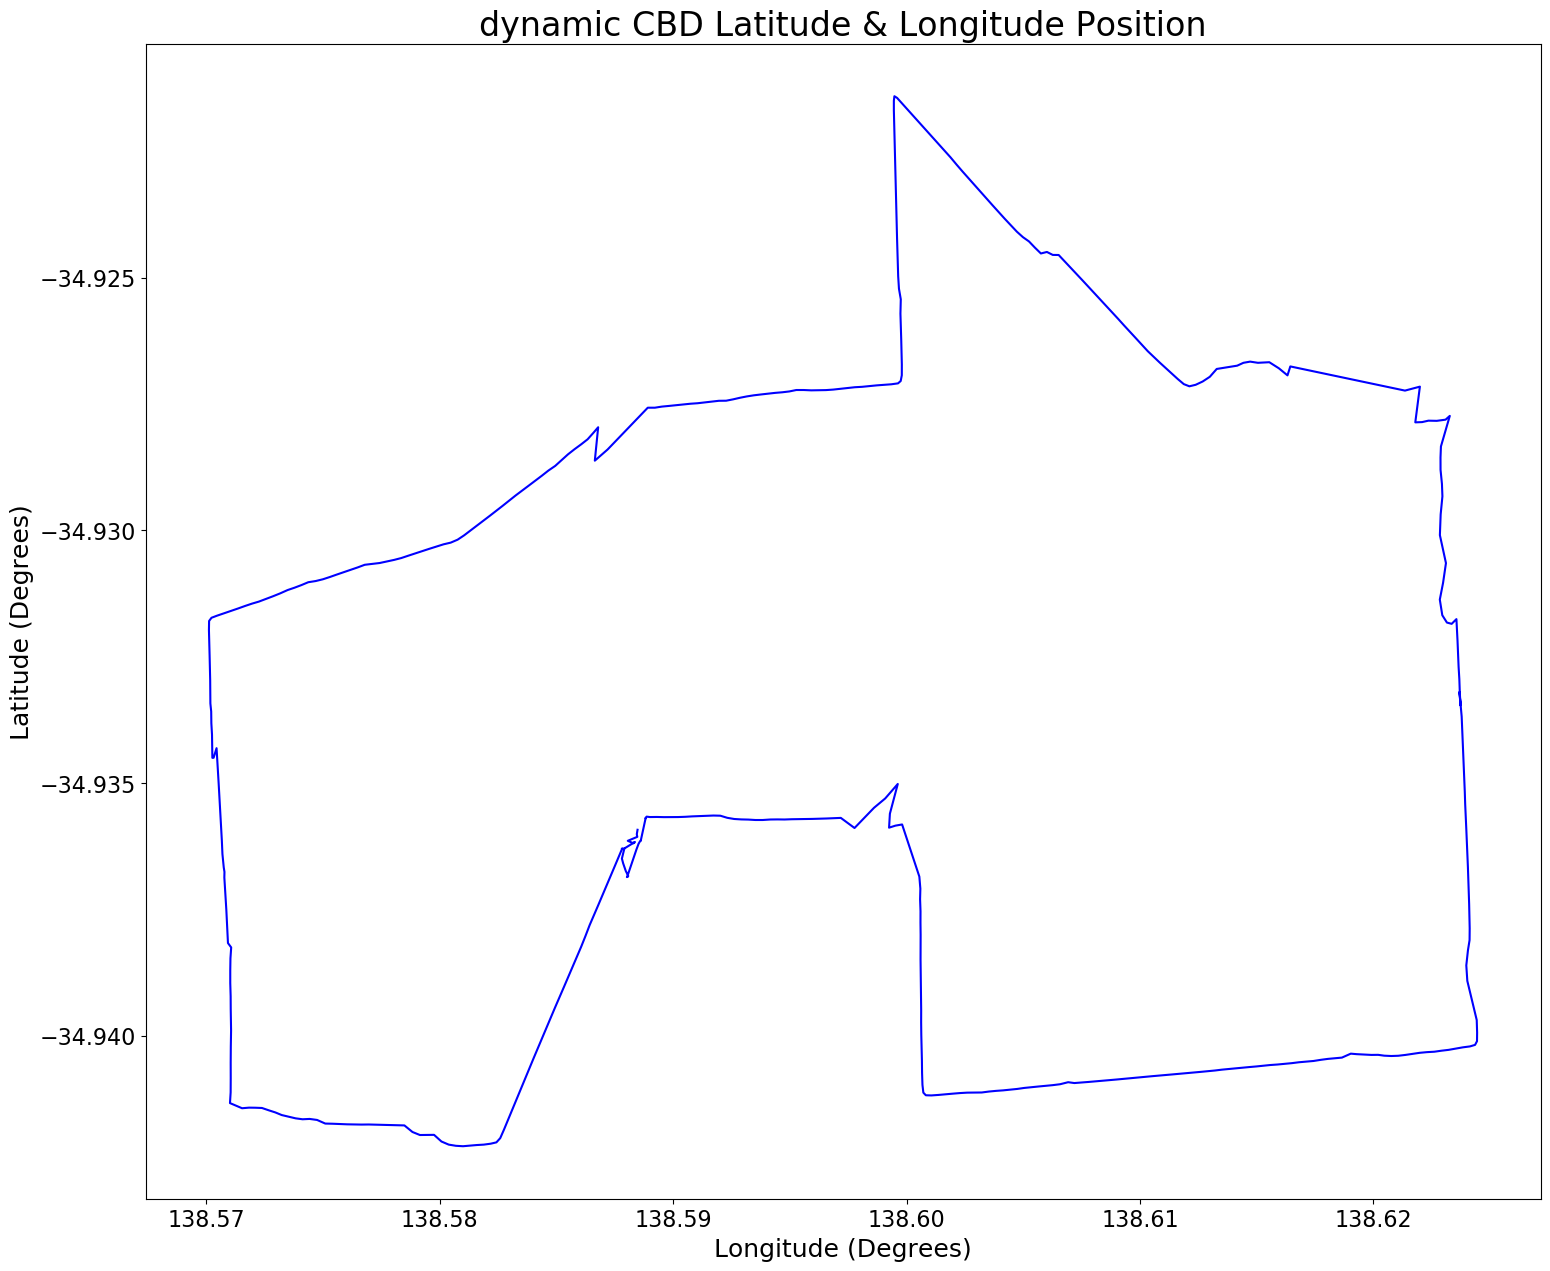
\includegraphics[width=12cm,keepaspectratio]{Figures/21_3_30_dynamic_CBD_results Lat long position.png}
        \caption{Trace of latitude and longitude over time as interpreted from the GPS receiver}
        \label{fig:CBDdynamicCoord}
    \end{centering}
\end{figure}

\begin{figure}[H]
    \begin{centering}
        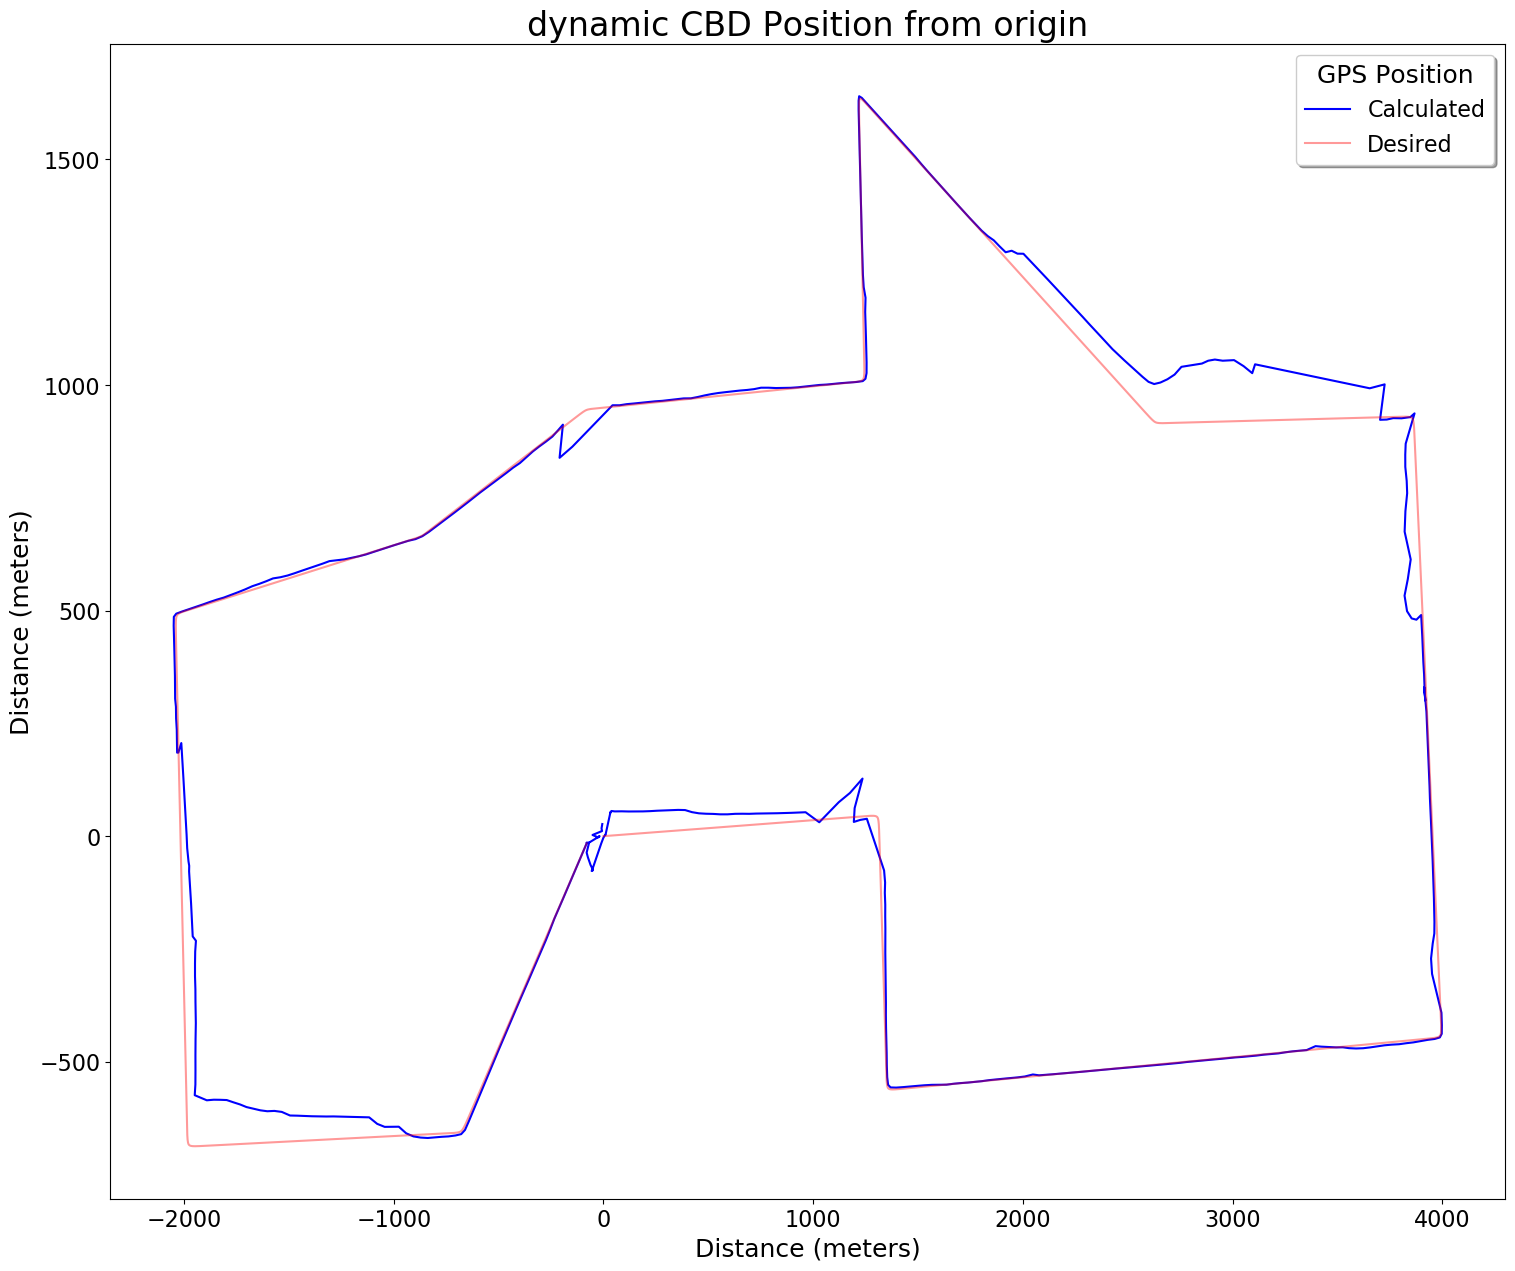
\includegraphics[width=12cm,keepaspectratio]{Figures/21_3_30_dynamic_CBD_results Position from origin.png}
        \caption{Graph of recorded position with respect to the reference location shown as a red path}
        \label{fig:CBDdynamicPosition}
    \end{centering}
\end{figure}

\begin{figure}[H]
    \begin{centering}
        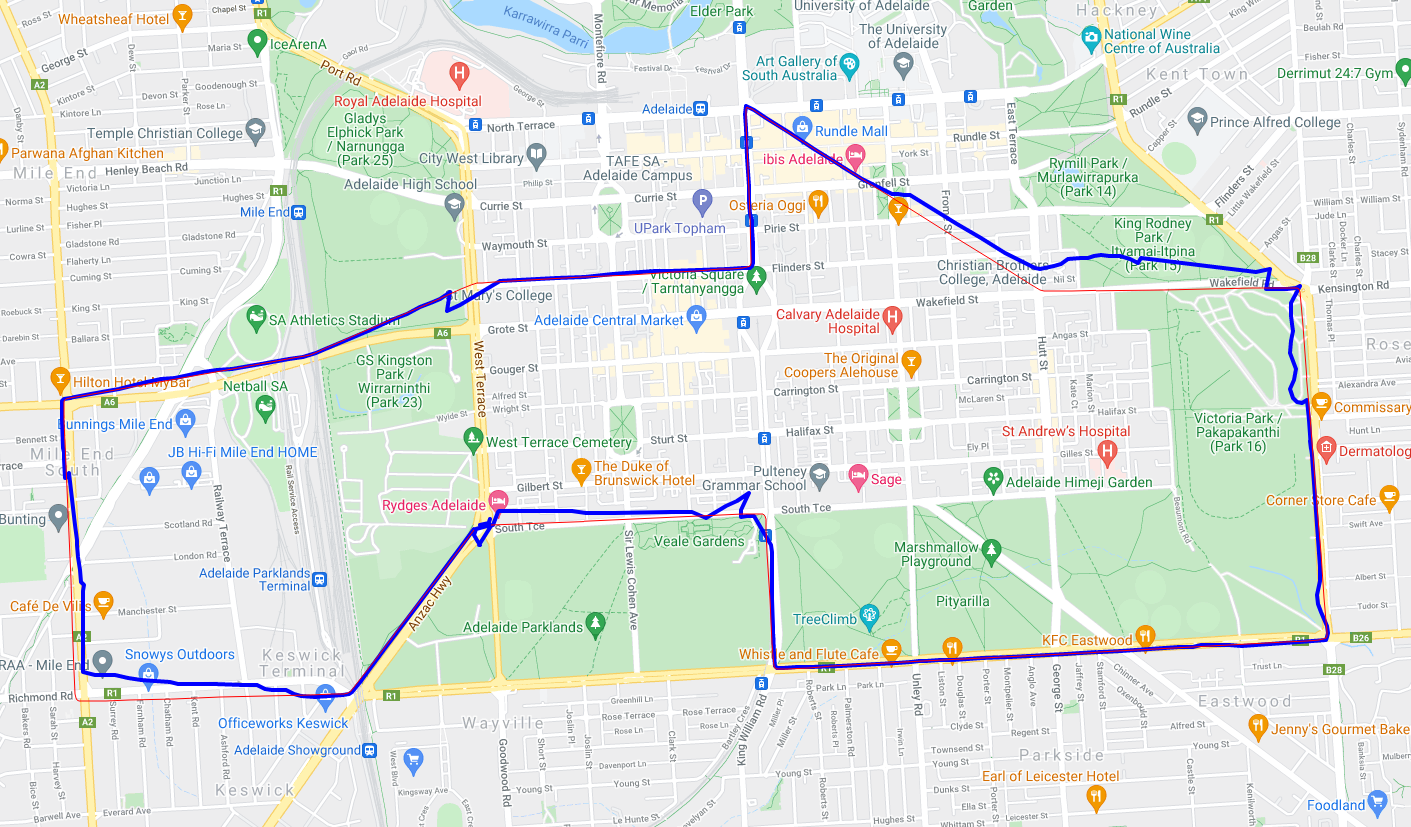
\includegraphics[width=14cm,keepaspectratio]{Figures/2021_3_30_dynamic_CBD_Satellite.PNG}
        \caption{Satellite image with expected GPS position shown with red cross and recorded position shown with blue line}
        \label{fig:CBDdynamicSatelliteImage}
    \end{centering}
\end{figure}

\section{Experimental Issues}
While performing experiments there were issues that were run into that were required to be overcome. Initially a Log Periodic antenna was used for transmission since its
frequency range was appropriate for use transmitting L1 band signals. After experiments failed to pick up any signals it was swapped for a omnidirectional antenna. The
antenna operating frequency was not known, though it's physical size seemed appropriate for the applicaiton. It was shown experimentally that is was
was able to produce signals that were picked up by the receivers. Observing the graphs of the carrier to noise figure showed that when there was an under run
issue the $\frac{C}{N_0}$ would drop to 0 and the GPS receiver would lose connection to the 'satellites'. This meant that no GPS lock was achievable.

The under run issue was solved by increasing the buffer size to $40\times$ greater than the sampling size, though there were still occasions where under run would still
occur. It was much less prominant after rebooting the PC.
There was an issue towards the end of the project where there was considerable leakage of EM radiation into the Faraday cage that was causing the GPS receiver to produce
wildly inaccurate position (up to and over 500m error). This was much different to what had previously been recorded within the Faraday cage. This amount of error does
not constitute a successful spoof since the time to first lock was much greater than a real signal, or even spoofing attempts previously. 

During initial testing of the spoofing there was an inability to get the spoofer to correctly spoof the receiver. It was found that there is a requirement that the ratio
between the sampling frequency and clock frequency of the radio must be an integer value. Therefore when compiling the signal using GPS-SDR-sim the sampling frequency
value was required to be changed to 2.5Msps.  

Just after the testing phase of the project the smartphone that was being used for some of the logging and graphing was rendered unusable. While there was no data lost,
it was replaced with a newer model that experimentally was much harder to spoof than the previous model. This could be due to many factors including anti-spoofing
algorithms \cite{RN39}. It would be a fair assessment that the newer device is able to receive more GNSS signals including augmented systems as well as other signals such as Wi-Fi.
The connection to the Wi-Fi signal was such that notifications were coming up on the phone while performing the experiments.

There were a number of unterminated cables that were running from outside of the cage to inside. This was seen as being the cause of the issues that were being faced. The
suspect cables were removed or terminated and the results were more consistent with what was being achieved previously. Even with the new phone the GPS location was able
to be spoofed.

A common result from spoofed attempts was to have GPS satellites with an SVID of 193. GPS satellites have PRN codes from 1-63 and SBAS have PRNs from
64 to 158 \cite{RN67}. From the list of PRN codes \cite{RN67} it can be seen that PRN 193 is used by one of the QZSS satellites. This is likely a result of stray EM waves
penetrating the Faraday cage. It is unlikely that the GPS-SDR-sim program includes augmentation systems when generating spoofed signals. The orbit of the QZSS satellites
does include Australia so seems most likely an issue where an unterminated cable is allowing the signal to bleed into the cage.

In an attempt to overcome the under run \todo{insert graph of under run}issue that was plaguing the experiments, a new PC was brought in with Ubuntu installed directly instead of via a VM. This resulted
in the radio working straight away. The under run issues resurfaced when trying to read the serial data from a COTS GPS receiver. This was less than ideal and required a
second computer to act as a datalogger.

\section{Discussion}
Initially it was decided that the locations that would be spoofed would be locations that are not easily accessible as a means of proving the validity of the results.
This was made easier due to the ongoing pandemic. Although this idea was later changed to make it easier to compare with real signals if needed.

Using the developed workflow, it was simple to create and deploy spoofing attacks for any location and at any elapsed time within minutes. This includes static or dynamic
spoofing attacks. Not enough time was invested into the reception of GNSS signals and thus meaconing attacks were not performed. The GPS-SDR-sim program was able to
estimate and simulate the ionic effects. While it is clear that this method resulted in successful spoofing attacks, the hypothesis is that having a received signal that includes ionic delays
and other interference would make it easier to fool more complicated receivers. Further testing and investigations should be carried out to find the answer to this. 

The results from the static Antarctica spoof attack, specifically the carrier to noise graphs show a high number of unique SVIDs. Based on the number of satellites in the
GPS constellation this must be an error. Although there was no explanation for the error since the resultant location was correct. One hypothesis was that the compilation
software added some incorrect data. Another is the prevalence of SBAS satellites. There was a known issue for some time with the Faraday cage where stray EM waves were
getting in. This would explain the consistency in which SVID 193 appears. From \cite{RN67} it can be seen that SVID 193 is a QZSS satellite. These satellites orbit over
Australia and part of Asia.

The dynamic spoof around the MAB showed low error while following the associate path. The CBD dynamic spoof, which lasted much longer, was less consistent with the
accuracy. There were sections where the error between desired and calculated location was high and secitons were it was close to ideal. This shows that over a long
transmission time the accuracy can fluctuate. This flucuation may be caused by the fluctuating values from the carrier to noise graph.

Consistently for both static and dynamic spoofing the $\frac{C}{N_0}$ ratio was a high value (between 40 and 50 dBHz). During experimentation it was found that authentic
GPS signals would be received with more variable $\frac{C}{N_0}$ ratio but with an average of around 30dBHz. This discrepancy can be attributed to a combination of the
controlled environment of the Faraday cage as well as the relative distance between the spoofer and victim. In theory the spoofed $\frac{C}{N_0}$ ratio could be higher,
but during compilation estimated Ionospheric effects are included. This shows that there is still room for improvement for the GPS-SDR-sim software, especially if it is
to be used in controlled environments for testing purposes. Just from the $\frac{C}{N_0}$ ratio graphs the spoofed signals are easy to identify.

On the $\frac{C}{N_0}$ ratio graphs there were consistently more SVIDs than expected. The trend was that static spoof attacks had more SVIDs than the dynamic spoofs, with
the most coming from the Antarctic spoof attack. It can also be seen that the length of attack was longest for the Antarctic spoof, which may account for this
discrepancy. Even still, the MAB static spoof included more than expected SVIDs.

SDRs are very sensitive to the processing pipeline of the computer that they are connected to. It is not uncommon to receive an under run error (where 'U' is printed to the
output) when transmitting a signal with high SPS (samples per second). This error is caused by the host computer not being able to feed the data to the radio quickly
enough.

This was solved by increasing the UDP buffer size manually to at least the sample rate, and over for better results. From limited experimentation this completely resolved the issue, and opened up
opportunities to perform spoofing with low powered embedded devices like the Raspberry Pi single board computer.
